% ============================================================
% MACROSCOPIC PHYSICS — ECT
% File: mp.tex
% Version: 10  (2026-03-16, pre-integration final)
%
% VERSION HISTORY:
%   v4:  §6.2 fully replaced — fixed metric formula g_eff^{AB}=β·δ-α·n·n;
%        Level A/B status split for metric vs φ-first closure
%   v5:  §6.3 FP-like wording; §6.4 schematic EMT_n; §6.5 derivation chain;
%        §6.6 Bianchi eq, homogeneous limit fix, neighbour-theory comparison
%   v6:  §6.7 two weak-field regimes; §6.8 D/c LIV fix (10^{-64} s);
%        §6.9 pre-Lorentzian scenario, V(Φ) inflaton language corrected;
%        §6.10 env. dependence g_†; §6.11 schematic lensing, exploratory BH;
%        §6.12 table updates (Pre-Lorentzian Level B, baryogenesis route)
%   v7:  FLRW Lambda_eff dimensional fix; r removed from §6.8 → §6.9;
%        §6.7 PPN estimate softened (no α²_PPN∼ε); citations added
%        (Bertotti2003, Uzan2011, Planck2018, DESI2024, Cromartie2019,
%        Riley2021, Lelli2016, McGaugh2016)
%   v8:  All 9 figures inserted with updated captions (timeline, cosmo,
%        w_z, sparc, MW, EFE, rar, gdagger, bullet_cluster)
%   v9:  §6.10 tab:phi_fits (6 galaxies), baryonic modelling, caveats
%        subsection added; figures/ paths verified
%   v10: Header updated for integration; all 4 deferred-basics sections
%        confirmed covered (sec:geom_branch, sec:noether, sec:spin2_content,
%        sec:GN_matching); pre-integration verification passed 15/15
%
% DISCIPLINE:
% (1) Every claim: Level A / B / EFT / matching / phenomenological / open.
% (2) Two parallel lines: mathematical + physical.
% (3) No import of hbar, Born rule, full QM.
% (4) Deferred basics subsections DEVELOPED here.
% (5) Old content preserved, improved, not shrunk.
% (6) Every strong claim \ref{} or \cite{}.
% (7) Comparisons with GR/BD/Einstein-aether preserved.
% (8) Numerical estimates tracked with status.
%
% INTEGRATION NOTE:
%   This file replaces the legacy Gravitational Sector, Lorentz-Order Field,
%   Rotation Curves, Cosmological Implications, and observational-tests sections
%   of ECT_preprint.tex. Upon integration, remove all legacy figure-blocks for:
%   fig:timeline, fig:cosmo_predictions, fig:w_z, fig:sparc_ect, fig:MW,
%   fig:EFE, fig:rar, fig:gdagger_analysis, fig:bullet_cluster
% ============================================================
% (1) Every claim: Level A / B / EFT / matching / phenomenological / open.
% (2) Two parallel lines: mathematical + physical.
% (3) No import of hbar, Born rule, full QM.
% (4) Deferred basics subsections DEVELOPED here.
% (5) Old content preserved, improved, not shrunk.
% (6) Every strong claim \ref{} or \cite{}.
% (7) Comparisons with GR/BD/Einstein-aether preserved.
% (8) Numerical estimates tracked with status.
% ============================================================

\section{Macroscopic Physics}
\label{sec:macroscopic}

% ============================================================
\subsection{Macroscopic Physics as the development
of the geometric branch}
\label{sec:mp_intro}
% ============================================================

\textit{Connection to ECT basics:
Sections~\ref{sec:branching}, \ref{sec:geom_branch}.
Status: conceptual bridge; all claims structural.}

\medskip
After completing ECT basics
(Sections~\ref{sec:postulates}--\ref{sec:branching}),
ECT is no longer an undifferentiated scheme.
As established in the branching section, after the selection of
the gradient-ordered vacuum sector and the restriction to the
coherent topological sector, the theory naturally separates into
two large effective branches.

\paragraph{Two branches from one condensate.}
The first branch---the \emph{geometric} or \emph{macroscopic}
branch~(\S\ref{sec:geom_branch})---describes those observables
that are insensitive to the local phase of the coherent order
parameter and are controlled instead by long-wavelength variations
of the ordered condensate background.
The second branch---the \emph{coherent-topological} or
\emph{Quantum Sector}~(\S\ref{sec:coh_branch})---describes
observables that probe the winding structure, loop sectors,
decoherence kernels, and quantum amplitudes of the coherent
order parameter $\Phi_{\rm eff}=\rho e^{i\theta}$.
The present section develops the first branch exclusively.

\paragraph{Definition of macroscopic observables.}
In ECT basics it was shown that after the $O(4)\to O(3)$
symmetry breaking, long-wavelength physics naturally separates
into a \emph{tensorial, phase-insensitive sector} and a
\emph{coherent-topological, phase-sensitive sector}.
The geometric branch is defined precisely by the former.
The primary variables of this branch are:
\begin{itemize}
  \item the effective metric $g^{\rm eff}_{AB}$, derived from the
    unique kinetic tensor $K^{AB}$~\eqref{eq:K_general};
  \item the orientation collective variable $n_A$~(P4);
  \item long-wavelength tensorial perturbations $\delta n_i$
    around the ordered vacuum~(Section~\ref{sec:mode_classes});
  \item conserved stress-energy structures from the
    variational/Noether foundation~(Section~\ref{sec:noether},
    Appendix~\ref{app:noether_full});
  \item the gravitational stiffness scale $M_G$, which controls
    matching to the observed Newton constant $G_N$.
\end{itemize}
None of these objects is introduced from scratch here: each
already appears in embryonic form in ECT basics, and Macroscopic
Physics is precisely its full development.

\paragraph{The coarse-graining criterion.}
The key transition from ECT basics to the macroscopic branch is
a coarse-graining over short-distance condensate structure.
The radial mode $\sigma$ with bare mass $m_\sigma=\sqrt{2\mu^2}$
(Section~\ref{sec:mode_classes}) sets the short-distance cutoff
of the ordered phase; the corresponding correlation length
$\xi_{\rm cond}\sim m_\sigma^{-1}$~(Appendix~\ref{app:corr_length})
marks the scale below which the condensate must be treated as a
structured medium rather than an effectively geometric background.
The macroscopic branch is therefore defined in the regime:
\begin{equation}
  \label{eq:macro_regime}
  L \gg \xi_{\rm cond}\sim m_\sigma^{-1},
  \qquad
  E \ll m_\sigma,
\end{equation}
where $L$ is the characteristic observational scale and $E$
the characteristic excitation energy.
In this limit the heavy radial mode is integrated out
(Appendix~\ref{app:eft_derivation}), rapid microscopic
phase fluctuations are averaged away, and the remaining
physically relevant variables are precisely the slow
orientation/background degrees of freedom~(Level~A:
this criterion follows directly from the EFT power counting
of Section~\ref{sec:mode_classes}).

\paragraph{Why the phase drops out.}
The macroscopic branch is defined not only by scale but by
the loss of sensitivity to local phase information.
In geometric-branch observables the phase $\theta$ of the
coherent order parameter $\Phi_{\rm eff}$ does not appear
explicitly; what remains are effective metric relations,
source couplings, causal propagation, and large-scale
background structure.
This is the fundamental reason why the present section develops
gravity, cosmology, and galactic phenomenology, while wave
amplitudes, canonical commutation relations, decoherence, and
probability measures are deferred to the Quantum Sector.

\paragraph{What is already established in ECT basics.}
From ECT basics the following is available for the geometric branch:
\begin{enumerate}[label=(\roman*)]
  \item three massless orientation modes $\delta n_i$ with dispersion
    $\omega^2=c_n^2 k^2$~(Section~\ref{sec:mode_classes},
    Appendix~\ref{app:sigma_model});
  \item Lorentzian window $\beta<\alpha<4\beta$~(Section~\ref{sec:lorentz_window});
  \item conserved $T^{AB}$ from translational invariance
    and angular currents $J^{C,AB}$ from $O(4)$-invariance
    ~(Section~\ref{sec:noether}, Appendix~\ref{app:noether_full});
  \item a gravitational stiffness scale $M_G$ was identified in ECT
    basics; its matching to $G_N$ is developed in Section~\ref{sec:mp_matching};
  \item structural compatibility with a Deser-type spin-2
    self-coupling route~(Section~\ref{sec:mode_hierarchy}).
\end{enumerate}

\paragraph{What does not follow automatically.}
The five points above do not automatically give:
the full nonlinear gravitational closure;
standard Einstein equations in final form;
complete matching of all phenomenological constants;
or any quantum-mechanical statement.
These are developed step by step below.

\paragraph{Logical order of the section.}
First: effective metric and macroscopic limit~(\S\ref{sec:mp_metric}).
Then: linear tensorial sector and propagation~(\S\ref{sec:mp_tensor}).
Next: Noether source structure and matter coupling~(\S\ref{sec:mp_noether}).
After: gravitational stiffness matching~(\S\ref{sec:mp_matching}).
Then: nonlinear closure~(\S\ref{sec:mp_nonlinear}).
Finally: weak-field limit, GWs, cosmology, galactic
phenomenology, observational tests
(\S\S\ref{sec:mp_newtonian}--\ref{sec:mp_tests}).

\paragraph{Physical picture.}
If ECT basics answers: \emph{what is the ordered medium and how
does it branch?}, then Macroscopic Physics answers:
\emph{how does the geometric branch of that medium appear to a
large-scale observer insensitive to coherent phase data?}
Gravity is not added to the condensate from outside; it is the
large-scale geometric response of the ordered condensate itself.

% ============================================================
\subsection{Effective metric and the macroscopic limit
of the condensate}
\label{sec:mp_metric}
% ============================================================

\textit{Status: Level~A for the emergence of the effective Lorentzian
metric structure in the broken-phase EFT~(Theorem~\ref{thm:tensor_uniqueness}).
The position-dependent coupling $G_{\rm eff}(X)=G_N e^{-\phi(X)}$
introduced below belongs to the phenomenological $\phi$-first closure
and is therefore Level~B.}

\medskip
The purpose of this subsection is to identify the minimal geometric
object that governs the macroscopic branch of ECT.
As established in ECT basics, once the vacuum sector has selected a
gradient-ordered background and the theory is restricted to long
wavelengths, the heavy radial mode decouples and the physically
relevant degrees of freedom are the slow orientation modes of the
ordered condensate.
However, this by itself does not yet determine which tensorial object
must be interpreted as the effective metric of the macroscopic branch.
We now show that, in the ordered phase, such a tensor arises uniquely
from the residual symmetry and that it acquires Lorentzian signature
for $\alpha>\beta$.

\subsubsection*{Coarse-graining and the macroscopic regime}

The macroscopic regime of ECT is defined not only by large distances,
but by coarse-graining over the microscopic structure of the ordered
condensate.
At the level of the bare microdynamics~(P3), the fundamental field
$\Phi$ and its gradient condensate retain an internal structure that
need not be geometric at ultrashort scales.
A geometric description becomes meaningful only after averaging over
regions much larger than the condensate correlation length
$\xi_{\rm cond}\sim m_\sigma^{-1}$~(Appendix~\ref{app:corr_length}).

Let $B_\ell(X)\subset\mathcal{M}^4$ be a neighbourhood of
characteristic size $\ell$ such that
\begin{equation}
  \label{eq:cg_regime}
  \xi_{\rm cond}\ll\ell\ll L,
  \qquad
  E\ll m_\sigma,
\end{equation}
where $L$ is the characteristic observational scale and $E$ the
characteristic excitation energy.
The coarse-grained orientation field:
\begin{equation}
  \label{eq:coarse_grained_n}
  \bar{n}_A(X)
  = \frac{1}{\mathcal{N}_\ell}
    \int_{B_\ell(X)}d^4Y\,W_\ell(X-Y)\,n_A(Y),
\end{equation}
where $W_\ell$ is a smooth window function localised at scale $\ell$
and $\mathcal{N}_\ell$ is the normalisation factor.
In the ordered phase $\bar{n}_A$ varies slowly:
\begin{equation}
  \label{eq:slow_orientation}
  |\partial_B\bar{n}_A|\ll\xi_{\rm cond}^{-1},
  \qquad
  |\partial_C\partial_B\bar{n}_A|\ll\xi_{\rm cond}^{-2}.
\end{equation}

Physically, the inequalities~\eqref{eq:cg_regime} define the regime
in which the condensate no longer behaves as a strongly structured
microscopic medium.
For $L\gg\xi_{\rm cond}$ and $E\ll m_\sigma$ the radial mode $\sigma$
is effectively integrated out~(Appendix~\ref{app:eft_derivation}),
and the remaining observables are controlled by slow orientation/background
variables.
This is the domain in which a metric description becomes natural.

\subsubsection*{Uniqueness of the macroscopic rank-2 tensor}

After spontaneous symmetry breaking $O(4)\to O(3)$, the only local
rank-2 tensors available in the ordered phase are the Euclidean tensor
$\delta_{AB}$ and the projector onto the preferred direction,
$\bar{n}_A\bar{n}_B$.
By Theorem~\ref{thm:tensor_uniqueness}~(Appendix~\ref{app:tensor_uniqueness}),
any symmetric rank-2 tensor compatible with the residual $O(3)$-symmetry
must have the form:
\begin{equation}
  \label{eq:K_macro}
  K^{AB}
  = \beta\,\delta^{AB} - \alpha\,\bar{n}^A\bar{n}^B.
\end{equation}
Introducing the orthogonal projectors
\begin{equation}
  \label{eq:projectors_macro}
  P_\parallel^{AB} = \bar{n}^A\bar{n}^B,
  \qquad
  P_\perp^{AB} = \delta^{AB} - \bar{n}^A\bar{n}^B,
\end{equation}
this becomes:
\begin{equation}
  \label{eq:K_macro_projector}
  K^{AB}
  = \beta\,P_\perp^{AB} - (\alpha-\beta)\,P_\parallel^{AB}.
\end{equation}
This is the macroscopic version of the tensor-uniqueness result
established in ECT basics~(\S\ref{sec:tensor_uniqueness}).

The effective metric is not inserted by hand.
The ordered phase admits one and only one symmetric rank-2 tensor
that (i)~survives coarse-graining, (ii)~respects the residual symmetry,
and (iii)~governs the principal part of long-wavelength propagation.
For this reason the geometric branch of ECT is not ``a field theory on
a chosen spacetime background'' but a theory in which the coarse-grained
response of the ordered condensate becomes interpretable as a metric.

\subsubsection*{Definition of the effective metric}

Since $K^{AB}$~\eqref{eq:K_macro_projector} controls the principal
part of long-wavelength equations of motion, it defines the causal and
metric structure of the macroscopic sector.
The effective inverse metric is identified as:
\begin{equation}
  \label{eq:geff_contra}
  g_{\rm eff}^{AB}
  = \beta\,P_\perp^{AB} - (\alpha-\beta)\,P_\parallel^{AB},
\end{equation}
equivalently written as:
\begin{equation}
  \label{eq:geff_contra_alt}
  g_{\rm eff}^{AB}
  = \beta\,\delta^{AB} - \alpha\,\bar{n}^A\bar{n}^B.
\end{equation}
Because $P_\perp$ and $P_\parallel$ are orthogonal projectors,
the covariant inverse metric is obtained exactly:
\begin{equation}
  \label{eq:geff_cov}
  g^{\rm eff}_{AB}
  = \frac{1}{\beta}\,P^\perp_{AB}
  - \frac{1}{\alpha-\beta}\,P^\parallel_{AB},
  \qquad
  g_{\rm eff}^{AC}g^{\rm eff}_{CB} = \delta^A{}_B.
\end{equation}

At this stage the effective metric is fixed only up to an overall
positive conformal factor—sufficient for determining causal structure
and the relative stiffness of longitudinal vs.\ transverse directions.
Overall normalisation is fixed later through matching
conditions~(\S\ref{sec:mp_matching}).

\subsubsection*{Lorentzian signature of the ordered phase}

Choose the local ordered frame $\bar{n}^A=(0,0,0,1)$.
Equation~\eqref{eq:geff_contra} then gives:
\begin{equation}
  \label{eq:geff_diag}
  g_{\rm eff}^{AB}
  = \operatorname{diag}\!\bigl(\beta,\,\beta,\,\beta,\,-(\alpha-\beta)\bigr).
\end{equation}
For $\alpha>\beta$ one eigenvalue changes sign and the effective metric
acquires Lorentzian signature.
At canonical normalisation $\alpha=2$, $\beta=1$:
$g_{\rm eff}^{AB}=\operatorname{diag}(1,1,1,-1)=\eta^{AB}$~(Level~A in EFT).

This is the precise mathematical form of the ``emergence of time'':
time is not introduced as an external coordinate but emerges as the
distinguished direction of the gradient-ordered condensate, identified
dynamically through the sign change of the kinetic tensor.

Defining $c_*^2=\beta/(\alpha-\beta)$~\eqref{eq:c_star_general} and
writing $w=c_*t$, the principal hyperbolic operator is:
\begin{equation}
  \label{eq:principal_op}
  g_{\rm eff}^{AB}\partial_A\partial_B
  = \beta\!\left(\nabla^2-\frac{1}{c_*^2}\partial_t^2\right)
  \propto \partial_t^2-c_*^2\nabla^2.
\end{equation}
This hyperbolic structure underlies retarded Green functions
(proved in Appendix~\ref{app:retarded_kernel}), causal cones, and
the tensorial propagation sector developed in \S\ref{sec:mp_tensor}.

\subsubsection*{Null structure and causal cones}

The effective null cones of the macroscopic branch:
\begin{equation}
  \label{eq:null_condition}
  g_{\rm eff}^{AB}k_Ak_B=0
  \quad\Longrightarrow\quad
  \beta\,\mathbf{k}^2-(\alpha-\beta)\,k_w^2=0
  \quad\Longrightarrow\quad
  \omega^2=c_*^2\,\mathbf{k}^2.
\end{equation}
Causal cones are emergent properties of the ordered condensate, not
primitive structures of the Euclidean arena.
For a macroscopic observer insensitive to coherent phase data,
the condensate appears as a Lorentzian medium: propagation is
hyperbolic, disturbances possess retarded response, and causal order
is reconstructed from the geometry of propagation.
This condensed-matter perspective on causality has precedents in
analogue gravity~\cite{Unruh1981,Volovik2003}.

\subsubsection*{Phenomenological $\phi$-first closure of the macroscopic branch}

The emergence of the effective metric above is a strict Level~A result.
By contrast, the introduction of a position-dependent effective Newton
coupling through a Lorentz-order field is part of the current
phenomenological closure of the macroscopic branch and is Level~B.

To parameterise slow background variations of the ordered branch, define
the dimensionless Lorentz-order field:
\begin{equation}
  \label{eq:phi_def}
  \phi(X)\equiv\ln\frac{\chi(X)}{\chi_\infty},
  \qquad \phi\big|_{\rm vac}=0,
\end{equation}
where $\chi(X)=\alpha(X)-\beta(X)$ characterises the local degree of
macroscopic ordering and $\chi_\infty$ is the background vacuum value.
In the phenomenological $\phi$-first closure:
\begin{equation}
  \label{eq:Geff_phi}
  G_{\rm eff}(X)=G_N\,e^{-\phi(X)}.
\end{equation}
This is not a completed first-principles theorem from bare P3; it is
the current ansatz connecting the strict Level~A effective Lorentzian
geometry to the Level~B phenomenological closure needed for
observational applications~(\S\S\ref{sec:mp_nonlinear}--\ref{sec:mp_tests}).

\subsubsection*{What is established and what is not}

\textbf{Established~(Level~A in broken-phase EFT):}
\begin{enumerate}[label=(\roman*)]
  \item The ordered phase admits a unique symmetric rank-2 tensor
    compatible with residual $O(3)$.
  \item This tensor controls the principal part of propagation and
    defines the effective inverse metric of the geometric branch.
  \item For $\alpha>\beta$ the effective metric has Lorentzian signature.
  \item The null structure and causal cones are emergent properties of
    the ordered condensate.
\end{enumerate}

\textbf{Not yet established:}
\begin{enumerate}[label=(\roman*)]
  \item $g^{\rm eff}_{AB}$ has not yet been identified with the complete
    physical metric of nonlinear GR.
  \item Conformal normalisation is not fixed by ECT basics alone.
  \item Matter coupling universality~(A4) is Level~B, not Level~A.
  \item $G_{\rm eff}(X)=G_N e^{-\phi}$ is a phenomenological ansatz,
    not a first-principles theorem.
\end{enumerate}

The correct status is therefore Level~A for the emergence of the
effective Lorentzian metric structure itself, and Level~B for the
phenomenological $\phi$-first closure used to connect that structure
to macroscopic applications.

\subsubsection*{Physical interpretation}

In the ordered phase the condensate ceases to be an isotropic Euclidean
medium.
One coarse-grained direction becomes dynamically distinguished by the
gradient condensate.
A macroscopic observer insensitive to phase information but sensitive
to propagation delays and source responses reconstructs a Lorentzian
spacetime not because it was postulated, but because the ordered
condensate acts as a medium whose tensorial response defines one.
The effective metric of ECT is thus a coarse-grained observable of the
ordered medium itself---not an external geometrical structure imposed
upon it~\cite{Volovik2003}.

\subsubsection*{Summary}

In the macroscopic limit the ordered phase generates an effective
Lorentzian metric:
\begin{equation}
  \label{eq:geff_summary}
  g_{\rm eff}^{AB}
  = \beta\,(\delta^{AB}-\bar{n}^A\bar{n}^B)
  - (\alpha-\beta)\,\bar{n}^A\bar{n}^B,
\end{equation}
unique by Theorem~\ref{thm:tensor_uniqueness}, defined up to conformal
normalisation, and governing the causal structure of the geometric branch.
This metric is the primary geometric object for all subsequent
subsections: linear tensor sector~(\S\ref{sec:mp_tensor}), Noether
sources~(\S\ref{sec:mp_noether}), matching of $M_G$~(\S\ref{sec:mp_matching}),
nonlinear closure~(\S\ref{sec:mp_nonlinear}), and phenomenological
applications~(\S\S\ref{sec:mp_newtonian}--\ref{sec:mp_tests}).


% ============================================================
\subsection{Linear tensor sector and the emergence
of gravitational propagation}
\label{sec:mp_tensor}
% ============================================================

\textit{Status: massless tensor propagation Level~A in EFT;
physical TT polarisations Level~B~(OP-gauge).
Migrated from: \texttt{sec:spin2\_content}, \texttt{app:sigma\_model}.}

\subsubsection*{Orientation modes as metric perturbations}

From the sigma-model analysis~(Appendix~\ref{app:sigma_model}),
the three soft orientation modes $\delta n_i$ satisfy:
\begin{equation}
  \label{eq:n_eom_macro}
  \partial_t^2\,\delta n_i - c_n^2\nabla^2\,\delta n_i = 0,
  \qquad \omega^2 = c_n^2 k^2,
  \qquad c_n\approx c_*
  \quad\text{(EFT matching)}.
\end{equation}
Through $g^{\rm eff}$~\eqref{eq:geff_summary}, these modes
induce metric perturbations $h_{\mu\nu}\propto\delta n_i$.
The resulting sector is a symmetric rank-2 tensor under $O(3)$
propagating at $c_n=c_*$~(Level~A in broken-phase EFT).

\paragraph{Physical meaning.}
The orientation modes $\delta n_i$ are the Goldstone bosons
of the spontaneous $O(4)\to O(3)$ breaking.
Their long-wavelength limit becomes gravitational wave propagation.
Gravity is the IR limit of the Goldstone sector of the broken
condensate, not a new ingredient.

\subsubsection*{Fierz--Pauli-like structure at linearised level}

On scales $L\gg\xi_{\rm cond}$, the quadratic action for metric perturbations can be organised
in a Fierz--Pauli-like form~\cite{Fierz1939}:
\begin{align}
  \label{eq:FP_action}
  S_{\rm FP} = M_G^2\int d^4x\,\bigl[
    \tfrac{1}{4}(\partial_\lambda h_{\mu\nu})^2
    - \tfrac{1}{4}(\partial_\lambda h)^2
    + \tfrac{1}{2}\partial_\mu h^{\mu\nu}\partial_\nu h
    - \tfrac{1}{2}(\partial_\lambda h^{\mu\nu})(\partial_\mu h_{\nu\lambda})
  \bigr],
\end{align}
where $h=\eta^{\mu\nu}h_{\mu\nu}$ and $M_G=\bar M_{\rm Pl}$
from Eq.~\eqref{eq:MG_def}~(Level~A for the existence of the linear tensorial kinetic structure
after coarse-graining; exact reducibility to the standard
Fierz--Pauli form remains part of OP-gauge/OP2).

\paragraph{Status of the two physical polarisations.}
If the macroscopic ECT tensor action is exactly reducible to
Fierz--Pauli form~\eqref{eq:FP_action}, then the usual linearised
gauge invariance
$h_{\mu\nu}\to h_{\mu\nu}+\partial_\mu\xi_\nu+\partial_\nu\xi_\mu$
would imply a reduction from 10 components to 2 physical TT modes.
\emph{This reducibility has not yet been demonstrated explicitly
in the ECT condensate language}~(OP-gauge).
Massless tensor propagation: Level~A in EFT;
exactly 2 TT modes: Level~B~(OP-gauge).

\paragraph{Comparison with Einstein-aether theory.}
In Einstein-aether theory~\cite{Jacobson2004} the unit vector
field~$u^A$ is a separate fundamental field.
In ECT, $n_A$ is a collective variable of the broken phase, not
in the bare action~P3.
The Fierz--Pauli structure emerges spontaneously, not by postulate.

\subsubsection*{Deser-compatible self-coupling route}

The structure established above satisfies the requirements of
Deser's self-coupling bootstrap~\cite{Deser1970}.
The geometric branch is therefore \emph{compatible with} a
Deser-type route to nonlinear Einstein equations~(Level~B; OP2).


% ============================================================
\subsection{Matter coupling and the Noether source structure}
\label{sec:mp_noether}
% ============================================================

\textit{Status: conservation laws Level~A; existence of a macroscopic
source tensor Level~A in the EFT; universality of matter coupling
Level~B~(OP-matter). The orientation-sector contribution to the
effective source structure can be written in an Einstein-aether-like
EFT form; the matching of its coefficients to the microscopic
condensate parameters remains Level~B/open~(OP2, OP-c1).
Migrated and expanded from: \texttt{sec:noether},
Appendix~\ref{app:noether_full}, and the deferred ECT basics notes.}

\medskip
The previous subsections established the effective metric structure of
the geometric branch and the existence of a linear tensorial propagation
sector.
The question now is: \emph{what plays the role of the gravitational
source in ECT?}
In general relativity the answer is the stress-energy tensor, which is
postulated to appear on the right-hand side of the Einstein equations.
In ECT the situation is conceptually different: the geometric branch is
not postulated from the outset as a spacetime theory but emerges from
the ordered condensate.
It must therefore be shown that the source structure arises
\emph{variationally} from the same condensate framework.

\subsubsection*{The variational origin of conserved source currents}

At the microscopic level the ECT action is local and does not depend
explicitly on the coordinates $X^A$ of the Euclidean arena~(P1, P3).
By Noether's theorem applied to translational invariance~\cite{Noether1918},
this yields a conserved rank-2 current for the scalar sector:
\begin{equation}
  \label{eq:Tab_Phi}
  T^{AB}_{(\Phi)}
  = \frac{\partial\mathcal{L}_\Phi}{\partial(\partial_A\Phi)}\,
    \partial^B\Phi - \delta^{AB}\mathcal{L}_\Phi,
  \qquad
  \partial_A T^{AB}_{(\Phi)} = 0
  \quad\text{(Level~A)}.
\end{equation}
The complete form including translational and rotational currents
is derived in Appendix~\ref{app:noether_full}.
After analytic continuation $w\to-ic_*t$ this becomes the standard
covariant conservation law $\nabla_\mu T^{\mu\nu}=0$.

This is a strict Level~A statement.
It depends only on the homogeneity of the Euclidean arena~(P1) and on
the locality of the action~(P3), not on any phenomenological closure.
The existence of a conserved source tensor in ECT is therefore not
borrowed from GR but intrinsic to the condensate's variational structure.

\paragraph{Caveat: time-dependent backgrounds.}
When the condensate background evolves in time (cosmological setting),
exact time-translation invariance is broken and global energy
conservation does not hold --- precisely as in GR with an evolving
metric~\cite{Weinberg1972}.
This is not a defect of ECT; it is structural consistency with the
GR-like limit.

\subsubsection*{From microscopic current to macroscopic source}

The tensor~\eqref{eq:Tab_Phi} is defined at the microscopic level.
The macroscopic branch requires a coarse-grained version.
Applying the same window function~\eqref{eq:coarse_grained_n}:
\begin{equation}
  \label{eq:Tab_coarse}
  \bar{T}^{AB}(X)
  = \frac{1}{\mathcal{N}_\ell}
    \int_{B_\ell(X)}d^4Y\,W_\ell(X-Y)\,T^{AB}(Y).
\end{equation}
Because averaging commutes with differentiation at long wavelengths:
\begin{equation}
  \label{eq:Tab_coarse_cons}
  \partial_A\bar{T}^{AB} = 0
  \quad\text{(up to higher-gradient corrections
  $\sim(\xi_{\rm cond}/L)^2$)}.
\end{equation}
The macroscopic source tensor of the geometric branch therefore remains
conserved~(Level~A in the coarse-grained EFT).

Physically, the macroscopic observer does not measure microscopic
gradients of $\Phi$ directly.
What is reconstructed are long-wavelength energy densities, momentum
fluxes, and stress-like components --- the hydrodynamic analogue of
the microscopic Noether current.

\subsubsection*{Orientation-sector contribution to the macroscopic source}

Beyond the pure scalar contribution~\eqref{eq:Tab_Phi}, the ordered
phase contributes an additional source component associated with the
orientation field $\bar{n}_A$.
At the level of the minimal sigma-model EFT~(Appendix~\ref{app:sigma_model}),
the corresponding source tensor has the schematic structure:
\begin{equation}
  \label{eq:EMT_n}
  T_{AB}^{(n)}
  = K_n\!\left[
    (\nabla_A n_C)(\nabla_B n^C)
    - \tfrac{1}{2}g_{AB}(\nabla_C n_D)(\nabla^C n^D)
  \right]
  + \lambda_n\,n_A n_B
  + \Delta_{AB}^{(n)},
\end{equation}
where $K_n$ is the orientation-sector stiffness~(related to $\kappa_n$,
Section~\ref{sec:mp_matching}), $\lambda_n$ enforces the normalisation
constraint on $n_A$, and $\Delta_{AB}^{(n)}$ collects additional
higher-derivative, curvature-coupled, or Einstein-aether-like
contributions appearing in more complete effective descriptions of
the ordered branch~\cite{Jacobson2004}.

The precise coefficient matching of $K_n$, $\lambda_n$, and the
subleading terms $\Delta_{AB}^{(n)}$ to the microscopic condensate
parameters of bare~P3 has not yet been completed.
Their correct status is therefore Level~B/open~(OP2, OP-c1).

This formulation is sufficient for the purposes of Macroscopic Physics:
it establishes that the ordered orientation sector contributes
nontrivially to the macroscopic source tensor, while leaving the full
first-principles completion to later work.

\subsubsection*{Rotational currents and the role of $O(4)$ symmetry}

From $O(4)$-invariance~(P2), Noether's theorem gives rotational currents:
\begin{equation}
  \label{eq:Noether_rotation}
  J^{C,AB}
  = X^A T^{CB} - X^B T^{CA} + S^{C,AB},
  \qquad
  \partial_C J^{C,AB} = 0
  \quad\text{(Level~A)},
\end{equation}
where $S^{C,AB}$ is the spin part (zero for the pure scalar sector).
In the ordered phase the collective variable $n_A$ induces a nontrivial
rotational current in the orientation sector.

The distinction between translational and rotational Noether structures
must be kept precise.
The conservation $\partial_A T^{AB}=0$ comes from \emph{translation}
invariance, not from $O(4)$ rotations.
The $O(4)$ symmetry instead constrains the tensorial form of the
ordered phase and produces the anisotropic corrections below.

\subsubsection*{Anisotropic source corrections}

Because the ordered phase is not isotropic, the macroscopic source
structure contains anisotropic corrections from the rotational Noether
sector.
In the effective Lorentzian language these take the form
(Appendix~\ref{app:curvature_coupling}):
\begin{equation}
  \label{eq:Theta_n}
  \Theta_{\mu\nu}[n]
  = c_1\!\left(
    n_\mu n^\lambda R_{\lambda\nu}
    + n_\nu n^\lambda R_{\lambda\mu}
    - \tfrac{1}{2}g_{\mu\nu}n^\alpha n^\beta R_{\alpha\beta}
  \right),
\end{equation}
where $c_1$ is a condensate-parameter-dependent coefficient~(OP-c1).
This tensor is absent from standard GR; in Einstein-aether
theory~\cite{Jacobson2004} an analogous term is postulated as a
fundamental coupling, whereas in ECT it arises variationally from
the rotational Noether structure of the ordered phase.
The comparison is instructive: the same structure that one theory must
postulate, the other derives from symmetry.

\subsubsection*{Why the source couples to the geometric branch}

The natural coupling of $\bar{T}^{AB}$ to the geometric branch follows
from the structure of the coarse-grained EFT.
The geometric branch is the phase-insensitive, tensorial sector of the
ordered condensate.
Its propagating excitations are the long-wavelength tensorial
deformations whose kinetic structure is governed by $g^{\rm eff}_{AB}$.
The only conserved rank-2 object available to source such deformations
is precisely the coarse-grained Noether tensor $\bar{T}^{AB}$.
The source coupling therefore follows from the EFT organisation, not
from a separate postulate~(Level~A for existence; Level~B for full
nonlinear coupling, see Section~\ref{sec:mp_nonlinear}).

\subsubsection*{Universality of matter coupling: current status}

A stronger claim is that \emph{all} slow matter sectors couple
universally to the same effective metric $g^{\rm eff}_{\mu\nu}$.
This is the analogue of the weak equivalence principle.
Within the present formulation it is a working assumption~(A4):
\begin{quote}
All matter sectors with $E\ll m_\sigma$ couple to the same
coarse-grained geometric structure $g^{\rm eff}_{\mu\nu}$.
\end{quote}
This is physically natural: once phase information is coarse-grained
away, the only macroscopic geometric data available to all slow sectors
is the same effective metric background.
Nevertheless, deriving this universality directly from bare P3 for
specific matter sectors has not yet been completed~(Level~B, OP-matter).

What is established at Level~A is the existence of a conserved
macroscopic source tensor and the natural coupling of the geometric
branch to that tensor.
What is not yet established at Level~A is the full universality of
matter coupling for arbitrary matter sectors.

\subsubsection*{Physical interpretation}

The Noether source structure of ECT carries a simple physical message:
the same condensate that generates the geometric branch also contains,
through its variational foundation, the conserved quantities that source
that branch.
There is no split between ``geometry'' and ``matter'' at the deepest
level.
Both are different long-wavelength aspects of the same ordered medium.

A macroscopic observer reconstructs the familiar language of gravity:
metric perturbations respond to stress-energy; causal propagation is
governed by the effective Lorentzian metric; matter distributions shape
the geometry of low-energy probes.
In ECT this structure is not postulated from the outset but
reconstructed from the variational and symmetry properties of the
ordered condensate.

\subsubsection*{What is established and what is not}

\textbf{Established (Level~A):}
\begin{enumerate}[label=(\roman*)]
  \item Conserved Noether tensor $T^{AB}$ from translational
    invariance~\eqref{eq:Tab_Phi}.
  \item Coarse-grained $\bar{T}^{AB}$ remains conserved in the
    long-wavelength regime~\eqref{eq:Tab_coarse_cons}.
  \item The geometric branch admits a natural coupling to a
    conserved rank-2 source tensor.
  \item Rotational currents $J^{C,AB}$ exist and generate
    anisotropic corrections~\eqref{eq:Theta_n}.
\end{enumerate}

\textbf{Open or conditional:}
\begin{enumerate}[label=(\roman*)]
  \item Full universality of matter coupling is Level~B~(OP-matter).
  \item Explicit nonlinear source structure beyond linear EFT:
    Section~\ref{sec:mp_nonlinear}.
  \item Coefficient $c_1$ not yet derived from first principles~(OP-c1).
  \item Matching of $K_n$, $\lambda_n$ to bare P3 condensate
    parameters~(OP2).
\end{enumerate}

\subsubsection*{Summary}

The macroscopic source structure of ECT follows from the variational
foundation of the ordered condensate.
Translational invariance provides the conserved source tensor
$T^{AB}$ and its coarse-grained counterpart $\bar{T}^{AB}$;
$O(4)$-rotational symmetry generates anisotropic corrections through
the orientation-sector current structure.
The coupling of the geometric branch to a source tensor is the only
variationally natural possibility in the coarse-grained EFT, not an
additional postulate.
This establishes the source side of macroscopic gravity in ECT and
prepares the ground for the matching of gravitational stiffness and
the status of the Newton constant in the next subsection.


% ============================================================
\subsection{Gravitational stiffness, Newton constant,
and the status of $G_N$}
\label{sec:mp_matching}
% ============================================================

\textit{Status: Level~A for the existence of a gravitational stiffness
scale in the linear tensor EFT; Level~B for its matching to the observed
Newton constant~$G_N$. Direct derivation of $M_G$ from the microscopic
condensate parameters of bare~P3 remains open~(OP2, OP3, OP-grad).
Migrated and rewritten from: \texttt{sec:GN\_matching} and the legacy
consistency-relations material.}

\medskip
The previous subsections established three ingredients of the geometric
branch: (i) an effective Lorentzian metric structure $g^{\rm eff}_{\mu\nu}$,
(ii) a linear tensorial propagation sector, and (iii) a conserved source
tensor.
The next question is: \emph{what sets the strength of gravitational
response in ECT?}
In standard relativistic language this is answered by the Newton constant
$G_N$ or equivalently the reduced Planck scale $\bar M_{\rm Pl}$.
In ECT the logically prior object is not $G_N$ itself but the
\emph{gravitational stiffness} of the ordered condensate, denoted~$M_G$.

\subsubsection*{Why a stiffness scale must exist}

Once the ordered branch supports long-wavelength tensorial deformations,
their quadratic effective action necessarily carries a coefficient with
dimension mass$^2$.
This coefficient measures how costly it is to deform the ordered
condensate geometry on macroscopic scales.
Exactly in this sense, the geometric branch possesses a stiffness.
Schematically:
\begin{equation}
  \label{eq:grav_stiffness_schematic}
  S_{\rm tens}^{(2)}
  \sim
  M_G^2 \int d^4x\,(\partial h)^2.
\end{equation}
The existence of such a coefficient is a Level~A EFT statement:
once a linear tensor sector exists, its quadratic action necessarily
contains a normalisation scale.
What is not yet fixed at Level~A is the numerical identification
of that scale with the observed gravitational coupling.

Physically, $M_G$ is the analogue of an elastic modulus of the ordered
condensate, but for geometric/tensorial deformations rather than for
ordinary lattice strain.
Large $M_G$ means that the condensate geometry is extremely stiff:
macroscopic curvature is generated only weakly by ordinary matter sources.
This is precisely what one expects from the observed weakness of gravity.

\subsubsection*{Definition of $M_G$ from the linear tensor sector}

The gravitational stiffness scale is defined by the overall coefficient
of the quadratic tensor kinetic term in the macroscopic EFT.
Using the Fierz--Pauli-like organisation of the linear tensor action
established in Section~\ref{sec:mp_tensor}:
\begin{equation}
  \label{eq:MG_def}
  M_G^2 = \bar M_{\rm Pl}^2
  = \frac{c_*^4}{8\pi G_N}
  \approx (2.435\times 10^{18}\,\text{GeV})^2
  \quad\text{(Level~B: EFT matching)}.
\end{equation}
Here $M_G$ is \emph{not} assumed to equal $\bar M_{\rm Pl}$ by definition.
Rather, it is the normalisation scale of the ECT tensor EFT, which is
then compared with observed weak-field gravity to fix its numerical value.

\subsubsection*{Matching to the observed Newton constant}

Comparison with linearised GR gives the macroscopic matching relation:
\begin{equation}
  \label{eq:GN_from_MG}
  G_N = \frac{c_*^4}{8\pi M_G^2}.
\end{equation}
This is a Level~B statement: a geometric EFT matching between the
macroscopic ECT tensor sector and the empirically known linear
gravitational response.
It must be read in the correct direction: observed gravity fixes the
numerical value of~$M_G$; ECT does not yet derive $G_N$ from bare P3.
Thus $M_G$ is the ECT quantity and $G_N$ is the measured constant
to which it is matched.

This methodological point matters.
In older formulations the temptation was to write down a direct formula
for $G_N$ from microscopic condensate parameters too early, before the
EFT logic was fully established.
In the present postulate-based reconstruction the geometric branch first
produces a stiffness scale, and only afterwards is that scale matched
to observed gravity.

\subsubsection*{Relation to the orientation-sector stiffness}

The appearance of $M_G$ is not arbitrary.
The ordered phase already contains, in the orientation sigma-model
(Appendix~\ref{app:sigma_model}), a stiffness coefficient $\kappa_n$
governing the soft orientation modes:
\begin{equation}
  \label{eq:sigma_kappa}
  S_n^{(2)}
  = \frac{\kappa_n}{2}
    \int d^4X\,(\partial_B\delta n_i)(\partial^B\delta n_i).
\end{equation}
Since $[\kappa_n]=\text{GeV}^2$ and $[M_G^2]=\text{GeV}^2$, dimensional
consistency suggests that both scales are related.
The minimal EFT estimate:
\begin{equation}
  \label{eq:MG_condensate}
  M_G^2 \sim c_M\,\kappa_n,
\end{equation}
where $c_M$ is a dimensionless matching coefficient of order unity.
This is not yet a derivation from microscopic parameters; it is an
intermediate bridge inside the ordered-branch EFT.
The exact value of $c_M$, and the dependence of $\kappa_n$ on
$(u_0,\alpha,\beta)$, remain open~(OP-grad, OP2).

\subsubsection*{Hierarchy of scales and the open derivation chain}

At present the correct hierarchy is:
\begin{itemize}
  \item the gradient vacuum scale $u_0$~(P4) characterises the ordered
    vacuum sector;
  \item the broken-phase kinetic anisotropy is controlled by
    $(\alpha,\beta)$;
  \item the orientation sigma-model carries stiffness $\kappa_n$;
  \item the macroscopic tensor sector carries stiffness $M_G$;
  \item observed gravity fixes $M_G$ through~\eqref{eq:MG_def}.
\end{itemize}
What is \emph{not} yet available is a strict first-principles chain:
\begin{equation}
  \label{eq:derivation_chain}
  (u_0,\alpha,\beta)
  \;\longrightarrow\; \kappa_n
  \;\longrightarrow\; M_G
  \;\longrightarrow\; G_N.
\end{equation}
That chain is one of the main open problems of the geometric branch.
Any formula directly identifying $M_G$ or $G_N$ with a simple algebraic
combination of $(u_0,\alpha,\beta)$ must therefore be treated as legacy
shorthand or phenomenological input unless explicitly rederived inside
the new EFT logic.

\subsubsection*{Connection to legacy notation}

Earlier versions of ECT used a single scale $v_0=\langle\Phi\rangle$
as shorthand for several conceptually distinct quantities.
In the present formulation this shorthand is abandoned; the relevant
objects are now clearly separated:
\begin{equation}
  \label{eq:scale_separation}
  \underbrace{\phi_0}_{\text{bare scalar min.}},
  \qquad
  \underbrace{u_0}_{\text{gradient-ordered scale}},
  \qquad
  \underbrace{\kappa_n}_{\text{orient.\ stiffness}},
  \qquad
  \underbrace{M_G}_{\text{grav.\ stiffness}}.
\end{equation}
No direct algebraic identification between legacy $v_0$ and the
new ordered-branch scales is assumed without explicit EFT derivation
(see terminological note in Section~\ref{sec:constants}).

\subsubsection*{Physical interpretation}

The weakness of gravity in ECT is interpreted as extreme stiffness of
the ordered condensate geometry.
Ordinary matter sources are far too weak to significantly deform the
ordered medium except over enormous scales.
Newton's constant does not measure a primitive force inserted by hand;
it measures the \emph{inverse macroscopic compliance} of the ordered
condensate geometry:
$G_N\propto M_G^{-2}$.
The smaller $G_N$ is, the larger $M_G$ is, and the harder it is to
bend the ordered medium.

\subsubsection*{Summary of statuses}

\begin{center}
\renewcommand{\arraystretch}{1.4}\small
\begin{tabular}{p{6.8cm}p{2.5cm}p{2.5cm}}
\hline\hline
Statement & Status & Basis \\
\hline
Gravitational stiffness scale $M_G$ exists in tensor EFT
  & Level~A & Linear tensor sector \\
$M_G$ matched numerically to $\bar M_{\rm Pl}$
  & Matched & Observational input \\
$G_N=c_*^4/(8\pi M_G^2)$: matching relation
  & Level~B & Comparison with lin.\ GR \\
$M_G=\bar M_{\rm Pl}$: numerical value
  & Matched & Observational input \\
$M_G^2\sim c_M\kappa_n$: EFT order-of-magnitude
  & Level~B & Dimensional analysis \\
$(u_0,\alpha,\beta)\to\kappa_n\to M_G$: derivation chain
  & Open & OP-grad, OP2 \\
$G_N$ from bare P3 without EFT input
  & Open & OP3 \\
\hline\hline
\end{tabular}
\end{center}




% ============================================================
% ============================================================
\subsection{Nonlinear closure of the geometric branch}
\label{sec:mp_nonlinear}
% ============================================================

\textit{Status: Level~A for the structural necessity of a nonlinear
macroscopic closure once the geometric branch contains
(i) an effective Lorentzian metric, (ii) a tensor propagation sector,
and (iii) a conserved source tensor.
Level~B for the explicit $\phi$-first nonlinear closure.
Lovelock uniqueness is Level~A only under assumptions A1--A5.
A first-principles derivation of the full nonlinear gravitational
sector directly from bare~P3 remains open~(OP2, OP3, OP-matter).}

\medskip
Sections~\ref{sec:mp_metric}--\ref{sec:mp_matching} established the
three ingredients that any macroscopic gravitational theory must
contain: an effective Lorentzian metric structure, a propagating tensor
sector, and a conserved source tensor.
The central question of this subsection is therefore:
\emph{what is the strongest nonlinear gravitational structure currently
justifiable within the ECT framework?}

\subsubsection*{Why nonlinear closure is unavoidable}

The need for nonlinear closure is not an extra hypothesis but a direct
consequence of the existence of the geometric branch itself.
If the ordered condensate admits (i) an effective metric controlling
causal propagation, (ii) a tensorial mode sector propagating on that
metric, and (iii) a conserved source tensor coupled to that sector,
then the response to finite-amplitude perturbations cannot be described
consistently by a purely linear theory.
The metric sector must self-interact, source terms must backreact on the
background, and the effective coupling must be closed at nonlinear level.

This statement is Level~A as a structural claim.
What is \emph{not} Level~A is the exact final form of that closure.
ECT at its current stage does not yet derive the full nonlinear metric
dynamics directly from bare~P3; instead it constrains the admissible
closure strongly and yields a natural phenomenological route:
the $\phi$-first closure of the macroscopic branch.

\subsubsection*{Why the closure is not taken to be pure GR immediately}

The geometric branch is not purely metric in origin.
It emerges from an ordered condensate that carries additional collective
information at the macroscopic level:
\begin{itemize}
  \item the orientation field $n_A$,
  \item the Lorentz-order field $\phi=\ln(\chi/\chi_\infty)$
    describing slow variations of the degree of ordering,
  \item anisotropic correction tensors $\Theta_{\mu\nu}[n]$
    from the rotational Noether sector~\eqref{eq:Theta_n}.
\end{itemize}
Therefore the most general nonlinear closure compatible with the present
state of ECT is not \emph{a priori} pure Einstein gravity, but an
effective scalar-tensor-orientation system whose homogeneous
pure-metric limit reduces to Einstein--Hilbert.
ECT does not claim that nonlinear GR has already been derived from P3.
What it claims is that the geometric branch narrows the admissible
closure to a very restricted class, and that the current best-developed
closure in that class is the $\phi$-first one.

\subsubsection*{Working assumptions of the $\phi$-first macroscopic closure}

\begin{description}[noitemsep,leftmargin=2.2em]
  \item[A1] \textbf{Ordered branch condition.}
    $\alpha>\beta$, so the effective metric has Lorentzian signature
    ~(Level~A, Sections~\ref{sec:ssb}, \ref{sec:mp_metric}).
  \item[A2] \textbf{IR locality.}
    Macroscopic dynamics at $E\ll m_\sigma$; closure truncated at local,
    two-derivative order.
  \item[A3] \textbf{Four-dimensional geometry.}
    Large-scale branch is four-dimensional~(P1 + ordered EFT).
  \item[A4] \textbf{Metric universality for slow matter.}
    Slow matter sectors couple to $g^{\rm eff}_{\mu\nu}$~(Level~B,
    OP-matter).
  \item[A5] \textbf{Pure-metric reduction.}
    When $\phi$ and $n_A$ are frozen, the closure reduces to a
    pure-metric two-derivative theory (Lovelock step only).
\end{description}
Assumptions A1--A3 belong to the established macroscopic EFT;
A4 is open but well-motivated; A5 is used only for the pure-metric limit.

\subsubsection*{The $\phi$-first effective IR action}

Under A1--A4, the strongest currently available nonlinear macroscopic
closure is:
\begin{equation}
  \label{eq:phi_first_action}
  S_{\rm IR}
  = \int d^4x\,\sqrt{-g}\,
  \left\{
    \frac{\bar M_{\rm Pl}^2}{2}\,e^\phi R
    - \frac{\bar M_{\rm Pl}^2}{2}\,\omega(\phi)\,(\partial_\mu\phi)^2
    - U(\phi)
    + \mathcal{L}_{\rm mat}[g_{\mu\nu},\Psi]
  \right\},
\end{equation}
where $e^\phi R$ expresses local modulation of gravitational response
by the degree of Lorentzian ordering; $\omega(\phi)(\partial\phi)^2$
governs slow dynamics of the order field; $U(\phi)$ is the macroscopic
effective potential; and $\mathcal{L}_{\rm mat}$ encodes matter sectors.
This action is Level~B.
Full derivation, comparison with GR/Brans--Dicke/Einstein-aether/Ho\v{r}ava--Lifshitz,
and Theorems A--F: Appendix~\ref{app:phi_first_EFE}.

\subsubsection*{Generalised Einstein equations}

Varying~\eqref{eq:phi_first_action} w.r.t.\ $g^{\mu\nu}$:
\begin{equation}
  \label{eq:gen_EE}
  e^\phi\!\left(R_{\mu\nu}-\tfrac{1}{2}g_{\mu\nu}R\right)
  + \Lambda_{\rm eff}(\phi)\,g_{\mu\nu}
  + \Theta_{\mu\nu}[\phi,n]
  = \frac{8\pi G_{\rm eff}(\phi)}{c^4}\,T_{\mu\nu}^{\rm mat},
\end{equation}
where $\Lambda_{\rm eff}(\phi)=U(\phi)/\bar M_{\rm Pl}^2$,
$G_{\rm eff}(\phi)=G_N e^{-\phi}$~\eqref{eq:Geff_phi},
and $\Theta_{\mu\nu}[\phi,n]$~\eqref{eq:Theta_n} collects derivative
and anisotropic correction terms from the order field and orientation
sector.
Equation~\eqref{eq:gen_EE} is the current best nonlinear field equation
of the geometric branch~(Level~B).

\subsubsection*{Bianchi consistency and source conservation}

Compatibility with the contracted Bianchi identity requires:
\begin{equation}
  \label{eq:bianchi_consistency}
  \nabla^\mu\!\left[
    e^\phi G_{\mu\nu}
    + \Lambda_{\rm eff}(\phi)\,g_{\mu\nu}
    + \Theta_{\mu\nu}[\phi,n]
  \right]
  = \nabla^\mu\!\left[
    \frac{8\pi G_{\rm eff}(\phi)}{c^4}\,T^{\rm mat}_{\mu\nu}
  \right].
\end{equation}
When $\phi$ or $n_A$ vary, this does not imply ordinary matter
conservation alone; it implies conservation of the \emph{total}
macroscopic source structure.
This is physically natural: matter, order-field gradients, and
anisotropic condensate contributions exchange energy-momentum
among themselves.
Ordinary GR appears only when the additional ordered-branch variables
are effectively frozen.

\subsubsection*{Homogeneous limit and recovery of Einstein gravity}

In the vacuum-normalised screened limit
\[
\phi\to 0,\qquad \nabla_\mu\phi=0,\qquad\Theta_{\mu\nu}\to 0,
\]
Eq.~\eqref{eq:gen_EE} reduces to standard Einstein equations with
cosmological constant:
\begin{equation}
  \label{eq:EE_standard}
  R_{\mu\nu}-\tfrac{1}{2}g_{\mu\nu}R
  + \Lambda_{\rm eff}\,g_{\mu\nu}
  = \frac{8\pi G_N}{c^4}\,T_{\mu\nu}^{\rm mat},
\end{equation}
with $\Lambda_{\rm eff}=U(\phi_0)/\bar M_{\rm Pl}^2$.
This shows that the ECT postulate structure does not push the theory
away from GR at large homogeneous scales; GR is the special regime
where additional macroscopic order variables are frozen or screened.

\subsubsection*{Lovelock uniqueness of the pure-metric limit}

Under A1--A5, Lovelock's theorem~\cite{Lovelock1971} applies:
in four dimensions, the unique local diffeomorphism-invariant
two-derivative pure-metric field equations are those of
Einstein--Hilbert gravity with cosmological constant.
\begin{quote}
  \textbf{Status:} Level~A \emph{under A1--A5}.
  It is a theorem that the pure-metric frozen-order reduction cannot be
  anything other than Einstein--Hilbert~+~$\Lambda$.
  It is \emph{not} a theorem that the full ECT geometric branch is
  always pure GR.
\end{quote}

\subsubsection*{Comparison with neighbouring theories}

\paragraph{General relativity.}
GR corresponds to the homogeneous screened limit of the ordered branch,
where $\phi$ and $n_A$ become dynamically invisible at macroscopic scales.

\paragraph{Brans--Dicke scalar-tensor theories.}
ECT shares an effective scalar modulating gravitational response.
But $\phi$ is not a new fundamental field; it is the macroscopic
Lorentz-order variable of the condensate branch.

\paragraph{Einstein--aether theory~\cite{Jacobson2004}.}
ECT shares a preferred-direction variable and anisotropic correction
tensors.
But the orientation field is not fundamental in the bare action~P3;
it is a collective variable of the ordered condensate phase.
This is the structural difference with Einstein-aether theories, which
postulate such a field from the outset.

\paragraph{Ho\v{r}ava--Lifshitz gravity.}
ECT also has an emergent preferred structure, but does not begin by
explicitly breaking Lorentz symmetry in the microscopic action.
The preferred macroscopic direction appears through spontaneous ordering
of the Euclidean arena.

\subsubsection*{Physical interpretation}

The nonlinear closure describes how the ordered condensate responds to
finite macroscopic deformations.
At linear level: propagating tensor modes.
At nonlinear level: full backreaction of matter, order gradients, and
anisotropic condensate structure on the emergent geometry.

Spacetime curvature is not an autonomous primitive field; it is the
nonlinear macroscopic deformation pattern of the ordered condensate.
The Einstein limit corresponds to the regime where the order field is
frozen and the medium appears purely metric.
Deviations from GR correspond to residual macroscopic signatures of the
underlying ordered structure.

\subsubsection*{What is established and what is not}

\textbf{Established or structurally fixed:}
\begin{enumerate}[label=(\roman*)]
  \item A nonlinear closure is \emph{required} once metric structure,
    tensor propagation, and source coupling all exist~(Level~A).
  \item The pure-metric two-derivative frozen-order limit is uniquely
    Einstein--Hilbert~+~$\Lambda$ in $d=4$~(Level~A under A1--A5).
  \item The current best-developed closure is the $\phi$-first one,
    Eq.~\eqref{eq:phi_first_action}~(Level~B).
\end{enumerate}

\textbf{Not yet established as first-principles theorems:}
\begin{enumerate}[label=(\roman*)]
  \item Full derivation of the nonlinear closure from bare~P3~(OP2).
  \item Microscopic derivation of $U(\phi)$~(OP3).
  \item Universality of matter coupling~(OP-matter).
  \item Exact nonlinear role of $\Theta_{\mu\nu}[n]$ in all
    regimes~(OP-c1).
\end{enumerate}

\subsubsection*{Summary}

The geometric branch of ECT requires a nonlinear completion.
The strongest currently available completion is the $\phi$-first
scalar-tensor closure~\eqref{eq:phi_first_action}--\eqref{eq:gen_EE},
whose homogeneous frozen-order limit reduces to standard Einstein
gravity with cosmological constant.
The full first-principles derivation of this nonlinear sector from
microscopic condensate dynamics remains open, but the EFT logic already
constrains the closure strongly.
This prepares the next stage: the weak-field limit and the emergence of
Newtonian and post-Newtonian gravity from the nonlinear geometric branch.


% ============================================================
\subsection{Weak-field and Newtonian limit}
\label{sec:mp_newtonian}
% ============================================================

\textit{Status: Level~A for the existence of a screened weak-field limit
recovering standard Newtonian gravity in the vacuum-normalised regime
$\phi\to 0$ with anisotropic corrections suppressed.
Level~B for the full weak-field phenomenology including $G_{\rm eff}(X)$,
order-field corrections, and the transition toward the galactic critical
branch.
This subsection prepares, but does not yet assume, the deep weak-field
critical regime developed in Section~\ref{sec:mp_galactic}.}

\medskip
The nonlinear closure of Section~\ref{sec:mp_nonlinear} establishes the
macroscopic field equations of the geometric branch.
The next task is to identify their weak-field limit and to show how
ordinary Newtonian gravity is recovered locally, while allowing
systematic departures at larger scales or lower accelerations.
This step is essential for two reasons: first, any viable macroscopic
closure must reproduce the well-tested Newtonian and post-Newtonian
regime in the Solar System; second, the same weak-field expansion
provides the entry point for the galactic phenomenology of
Section~\ref{sec:mp_galactic}.

\subsubsection*{Weak-field expansion of the geometric branch}

We consider the macroscopic branch in the regime:
\begin{equation}
  \label{eq:weak_field_expansion}
  g_{\mu\nu}=\eta_{\mu\nu}+h_{\mu\nu},
  \qquad |h_{\mu\nu}|\ll 1,
  \qquad |\phi|\ll 1,
  \qquad v\ll c_*,
\end{equation}
around the vacuum-normalised ordered background
$\phi=0$, $\bar{n}_A=(0,0,0,1)$, with the quasi-static approximation
for nonrelativistic sources:
\begin{equation}
  \label{eq:quasistatic}
  |\partial_t|\ll c_*|\nabla|,
  \qquad T_{00}\gg T_{0i},\,T_{ij}.
\end{equation}
In Newtonian gauge:
\begin{equation}
  \label{eq:newtonian_gauge}
  ds^2 = -(1+2\Psi)c^2dt^2 + (1-2\Phi)\delta_{ij}dx^idx^j.
\end{equation}
In pure GR with negligible anisotropic stress one has $\Phi=\Psi$.
In ECT this equality is recovered in the screened local regime;
small deviations appear when the order field or orientation corrections
become dynamically relevant.

\subsubsection*{Screened local limit: recovery of Newtonian gravity}

In the locally screened vacuum-normalised regime:
\[
\phi\simeq 0,\qquad \nabla\phi\simeq 0,\qquad \Theta_{\mu\nu}[n]\simeq 0.
\]
The generalised field equations~\eqref{eq:gen_EE} reduce to the
standard Poisson equation:
\begin{equation}
  \label{eq:Poisson_standard}
  \nabla^2\Psi = 4\pi G_N\rho_{\rm bar},
  \qquad \Phi=\Psi.
\end{equation}
In the same limit the post-Newtonian parameter:
\begin{equation}
  \label{eq:PPN_gamma}
  \gamma_{\rm PPN}\equiv\frac{\Phi}{\Psi}\simeq 1,
\end{equation}
as in GR, consistent with the Cassini bound
$|\gamma_{\rm PPN}-1|<2.3\times10^{-5}$~\cite{Bertotti2003}.

This recovery is the key local consistency requirement of ECT
Macroscopic Physics.
Its status is Level~A conditional on the screened vacuum-normalised weak
limit: once the geometric branch exists and local order variables are
frozen, ordinary Newtonian gravity follows.

\subsubsection*{Weak-field form of the $\phi$-first closure}

Outside the fully screened regime but still in the quasi-static
weak-field domain, the $\phi$-first closure leads to:
\begin{equation}
  \label{eq:mod_Poisson}
  \nabla^2\Psi(X)
  \simeq
  4\pi G_{\rm eff}(X)\,\rho_{\rm bar}(X)
  + \mathcal{D}_{\phi,n}(X),
  \qquad
  G_{\rm eff}(X) = G_N e^{-\phi(X)},
\end{equation}
where $\mathcal{D}_{\phi,n}$ summarises residual derivative and
anisotropic source terms of the order field and orientation sector.
This is Level~B: the consistent weak-field reduction of the $\phi$-first
closure, not yet a first-principles theorem from bare~P3.

\paragraph{Observational bounds on $\dot G$.}
If the weak-field configuration evolves slowly in time:
\begin{equation}
  \label{eq:Gdot_over_G}
  \frac{\dot G_{\rm eff}}{G_{\rm eff}} = -\dot\phi.
\end{equation}
Lunar laser ranging gives $|\dot G/G|\lesssim 10^{-12}$\,yr$^{-1}$~\cite{Uzan2011},
requiring $|\dot\phi|\lesssim 10^{-12}$\,yr$^{-1}$, fully consistent
with a quasi-static screened condensate background~(Level~B).

\subsubsection*{Order-of-magnitude estimates for local deviations from GR}

Define the dimensionless deviation from the vacuum-normalised branch:
\begin{equation}
  \label{eq:epsilon_dev}
  \varepsilon(X)\equiv e^{-\phi(X)}-1\approx -\phi(X)
  \qquad\text{for }|\phi|\ll 1.
\end{equation}
Then one expects, at order of magnitude,
\[
\frac{\delta G}{G}\sim\varepsilon,
\]
while post-Newtonian deviations are likewise controlled by the same
small screening parameter.
Requiring consistency with Solar-System bounds motivates:
\begin{equation}
  \label{eq:epsilon_local_bound}
  |\varepsilon_{\rm local}|\lesssim 10^{-5},
  \qquad
  |\phi_{\rm local}|\lesssim 10^{-5},
\end{equation}
as a representative local screening condition.
The precise mapping to the full post-Newtonian parameter set remains
part of the detailed weak-field phenomenology and is therefore Level~B.

\subsubsection*{Two weak-field regimes of the geometric branch}

The new ECT architecture makes explicit that the weak-field domain
splits into two physically distinct subregimes:

\paragraph{(a) Screened local weak-field branch.}
$\phi\simeq 0$, $\Theta_{\mu\nu}\simeq 0$: GR/Newtonian physics is
recovered to high precision.
Relevant for Solar System and laboratory gravity.

\paragraph{(b) Deep weak-field ordered branch.}
The metric perturbation remains small, but order-sector corrections
become competitive with or dominant over the baryonic Newtonian source.
This is the regime in which $G_{\rm eff}(X)$ and the critical branch of
$\phi$-dynamics modify rotation curves, RAR, and BTFR phenomenology.
Developed in Section~\ref{sec:mp_galactic}.

This split is a real conceptual improvement over older ECT versions,
which treated ``the weak-field limit'' as a single regime.
The new postulate logic shows there are two weak-field regimes, separated
not by the size of the metric perturbation alone, but by the dynamical
state of the ordered branch.

\subsubsection*{Physical interpretation}

In ECT, a baryonic mass distribution sources a deformation of the
ordered macroscopic branch; the Newtonian potential is the screened local
projection of that deformation.
In the local branch the ordered medium responds almost rigidly, recovering
standard Newtonian gravity.
In the deep weak-field branch the medium is still weakly curved but no
longer fully screened, and residual order-sector structure becomes
visible.
This is why ECT remains compatible with Solar-System precision tests
while leaving room for nontrivial galactic phenomenology.

\subsubsection*{What is established and what is not}

\textbf{Established (Level~A in screened limit):}
\begin{enumerate}[label=(\roman*)]
  \item A screened weak-field limit of the geometric branch exists.
  \item Standard Poisson gravity is recovered in that limit.
  \item The weak-field domain splits structurally into screened local
    and deep weak-field ordered regimes.
\end{enumerate}

\textbf{Level~B / open:}
\begin{enumerate}[label=(\roman*)]
  \item Detailed form of $\mathcal{D}_{\phi,n}$ in all environments.
  \item Full post-Newtonian parameter set beyond $\gamma_{\rm PPN}$.
  \item First-principles microscopic derivation of screening
    from bare~P3.
\end{enumerate}

\subsubsection*{Summary}

The weak-field limit of the geometric branch is not a single universal
regime but a hierarchy.
In the screened local branch ECT reproduces standard Newtonian gravity.
In the $\phi$-first weak-field branch the Newtonian potential obeys a
modified Poisson equation with both baryonic and order-sector
contributions.
This is the bridge between the nonlinear macroscopic closure and the
galactic critical branch of Section~\ref{sec:mp_galactic}.



% ============================================================
% ============================================================
\subsection{Gravitational waves and causal structure}
\label{sec:mp_gw}
% ============================================================

\textit{Status: GW propagation speed Level~A in broken-phase EFT;
polarisation content Level~B~(OP-gauge);
Planck-suppressed LIV correction estimate Level~A in EFT
power-counting once a propagation distance~$D$ is specified.}

\subsubsection*{Propagation speed}

From the massless tensor dispersion relation~\eqref{eq:n_eom_macro},
the GW propagation speed equals the effective causal speed of the
ordered branch:
\begin{equation}
  \label{eq:cgw}
  c_{\rm GW}=c_n=c_*
  \quad\text{(Level~A at the benchmark }\alpha=2\beta\text{)}.
\end{equation}
Consistent with $|c_{\rm GW}/c-1|<6\times10^{-15}$ from GW\,170817
and its electromagnetic counterpart~\cite{LIGO_Virgo_GW170817_2017}.

\subsubsection*{Planck-suppressed Lorentz-violation estimate}

Because Lorentz symmetry is emergent rather than fundamental in ECT,
the leading high-energy correction to GW propagation is
Planck-suppressed in the EFT:
\begin{equation}
  \label{eq:gw_liv_dispersion}
  \omega^2 = c_*^2 k^2
  \left[1+\xi_2\!\left(\frac{k}{M_{\rm LIV}}\right)^2
  + O\!\left(\frac{k^4}{M_{\rm LIV}^4}\right)\right],
\end{equation}
where $\xi_2\sim O(1)$ and $M_{\rm LIV}\sim\bar M_{\rm Pl}$.
Induced fractional group-velocity shift:
\begin{equation}
  \label{eq:gw_velocity_shift}
  \frac{\delta v_{\rm GW}}{c}
  \sim \xi_2\!\left(\frac{E_{\rm GW}}{M_{\rm LIV}}\right)^2.
\end{equation}
Arrival-time shift over propagation distance~$D$:
\begin{equation}
  \label{eq:LIV_gw}
  \Delta t_{\rm GW}
  \sim \frac{D}{c}\,\xi_2
    \!\left(\frac{E_{\rm GW}}{M_{\rm LIV}}\right)^2.
\end{equation}
For GW170817-like parameters ($D\sim40$\,Mpc,
$E_{\rm GW}\sim4\times10^{-13}$\,eV,
$M_{\rm LIV}\sim\bar M_{\rm Pl}$):
\begin{equation}
  \label{eq:gw_liv_numeric}
  \Delta t_{\rm GW}\sim\xi_2\times10^{-64}\,\text{s}
  \quad\text{(negligible observationally)}.
\end{equation}

\subsubsection*{Polarisation content}

The orientation sigma-model provides three soft modes $\delta n_i$.
Full reduction to physical propagating content requires gauge analysis
(OP-gauge):
\begin{itemize}
  \item massless tensor propagation sector: Level~A;
  \item exact reduction to 2 TT polarisations: Level~B~(OP-gauge).
\end{itemize}
The anisotropic correction $\Theta_{\mu\nu}[n]$~\eqref{eq:Theta_n}
may additionally modify amplitude evolution in nontrivial ordered
backgrounds~(Level~B; OP-c1).

\subsubsection*{What is established and what is not}

\textbf{Established:}
\begin{enumerate}[label=(\roman*)]
  \item $c_{\rm GW}=c_*$~(Level~A).
  \item LIV correction is Planck-suppressed; induced delay
    $\Delta t\lesssim10^{-64}$\,s is negligible.
\end{enumerate}

\textbf{Open:}
\begin{enumerate}[label=(\roman*)]
  \item Exact 2 TT polarisations~(OP-gauge).
  \item Polarisation effects from $\Theta_{\mu\nu}[n]$~(OP-c1).
  \item Full radiative stability at loop level.
\end{enumerate}

% ============================================================
\subsection{Cosmological branch of the macroscopic sector}
\label{sec:mp_cosmo}
% ============================================================

\textit{Status: the whole subsection is Level~B unless stated
otherwise. The existence of a pre-Lorentzian Euclidean regime is a
structurally motivated cosmological scenario suggested by P1--P4, not
yet a completed first-principles cosmological theorem. $U(\phi)$
remains open~(OP3).}

\subsubsection*{A pre-Lorentzian Euclidean regime as a cosmological
scenario}

ECT naturally suggests a cosmological scenario in which the Universe
passes through a pre-Lorentzian regime before the ordered branch is
fully established.
In that regime there is no gradient-ordered vacuum sector, no effective
Lorentzian metric, and no preferred temporal direction.
This is strongly motivated by P1--P4, but the actual cosmological
realisation remains Level~B:
it is a structural scenario, not a theorem derived from completed
nonequilibrium condensate dynamics.
What ECT \emph{does} establish structurally is that macroscopic time is
not fundamental; therefore a cosmological history in which
time-bearing Lorentzian geometry appears only after the ordering
transition is natural in ECT in a way it is not in standard
GR-based cosmology.


% --- fig:timeline ---
\begin{figure}[H]
\centering
\includegraphics[width=\textwidth]{figures/fig5_ECT_timeline_condensate.png}
\caption{Schematic cosmological history in the ECT macroscopic branch.
\textbf{Top row~(a):} standard $\Lambda$CDM-style timeline.
\textbf{Bottom row~(b):} ECT-inspired ordering scenario in which a
pre-Lorentzian Euclidean regime precedes the emergence of the ordered
Lorentzian branch.
The transition $O(4)\to O(3)$ is shown schematically as the stage at
which macroscopic temporal direction and Lorentzian causal structure
become established.
Inflation is interpreted here as an effective ordering transition,
not yet as a first-principles theorem from bare~P3.
\textbf{Panel~(c):} schematic evolution of coarse-grained ordering and
macroscopic cosmological quantities.
If legacy notation appears inside the plot, it should be read as
historical shorthand rather than as the new postulate-level parameter
hierarchy.}
\label{fig:timeline}
\end{figure}

\subsubsection*{Homogeneous FLRW branch after ordering}

Once the ordered geometric branch is established on large scales, the
effective metric reduces to an FLRW form.
In the homogeneous $\phi$-first closure:
\begin{equation}
  \label{eq:FLRW}
  H^2
  = \frac{8\pi G_N}{3}\,\rho_{\rm mat}
  + \frac{\Lambda_{\rm eff}(\phi_0)}{3},
  \qquad
  \Lambda_{\rm eff}(\phi_0)=\frac{U(\phi_0)}{\bar M_{\rm Pl}^2}.
\end{equation}
Equivalently, defining the effective vacuum energy density
$\rho_{\Lambda,{\rm eff}}=U(\phi_0)$:
\[
H^2=\frac{8\pi G_N}{3}\!\left(\rho_{\rm mat}+\rho_{\Lambda,{\rm eff}}\right).
\]
This is the cosmological reduction of the macroscopic closure
\eqref{eq:phi_first_action}--\eqref{eq:gen_EE}, not a derivation from
bare~P3.

\subsubsection*{Inflation as an ordering transition}

In the ECT picture, inflation is naturally interpreted as the
macroscopic ordering transition by which the Lorentzian branch becomes
established, driven by an \emph{effective order-field potential} rather
than directly by the bare P3 potential.
If one adopts a slow-roll effective closure of plateau type:
\begin{equation}
  \label{eq:inflation}
  n_s \approx 1-\frac{2}{N_e}\approx 0.967,
  \qquad
  r \approx \frac{12}{N_e^2}\approx 0.003
  \quad (N_e\approx 60),
\end{equation}
consistent with Planck~2018~\cite{Planck2018}: $n_s=0.9649\pm 0.0042$.
Status: Level~B --- predictions of an effective inflationary closure,
not outputs of bare P3.

\subsubsection*{Dark energy as residual order-field vacuum energy}

The effective potential $U(\phi)$ generically has a residual nonzero
value at $\phi=0$.
In the macroscopic Einstein form this corresponds to:
\begin{equation}
  \label{eq:dark_energy}
  \Lambda_{\rm eff}=\frac{U(0)}{\bar M_{\rm Pl}^2},
  \qquad
  \rho_{\Lambda,{\rm eff}}=U(0).
\end{equation}
A representative phenomenological fit in the current closure:
\begin{equation}
  \label{eq:w0_fit}
  w_0\approx -0.83
  \quad\text{(Level~B; closure-dependent benchmark,
  consistent with DESI~2024~\cite{DESI2024})}.
\end{equation}


% --- fig:w_z ---
\begin{figure}[htb]
\centering
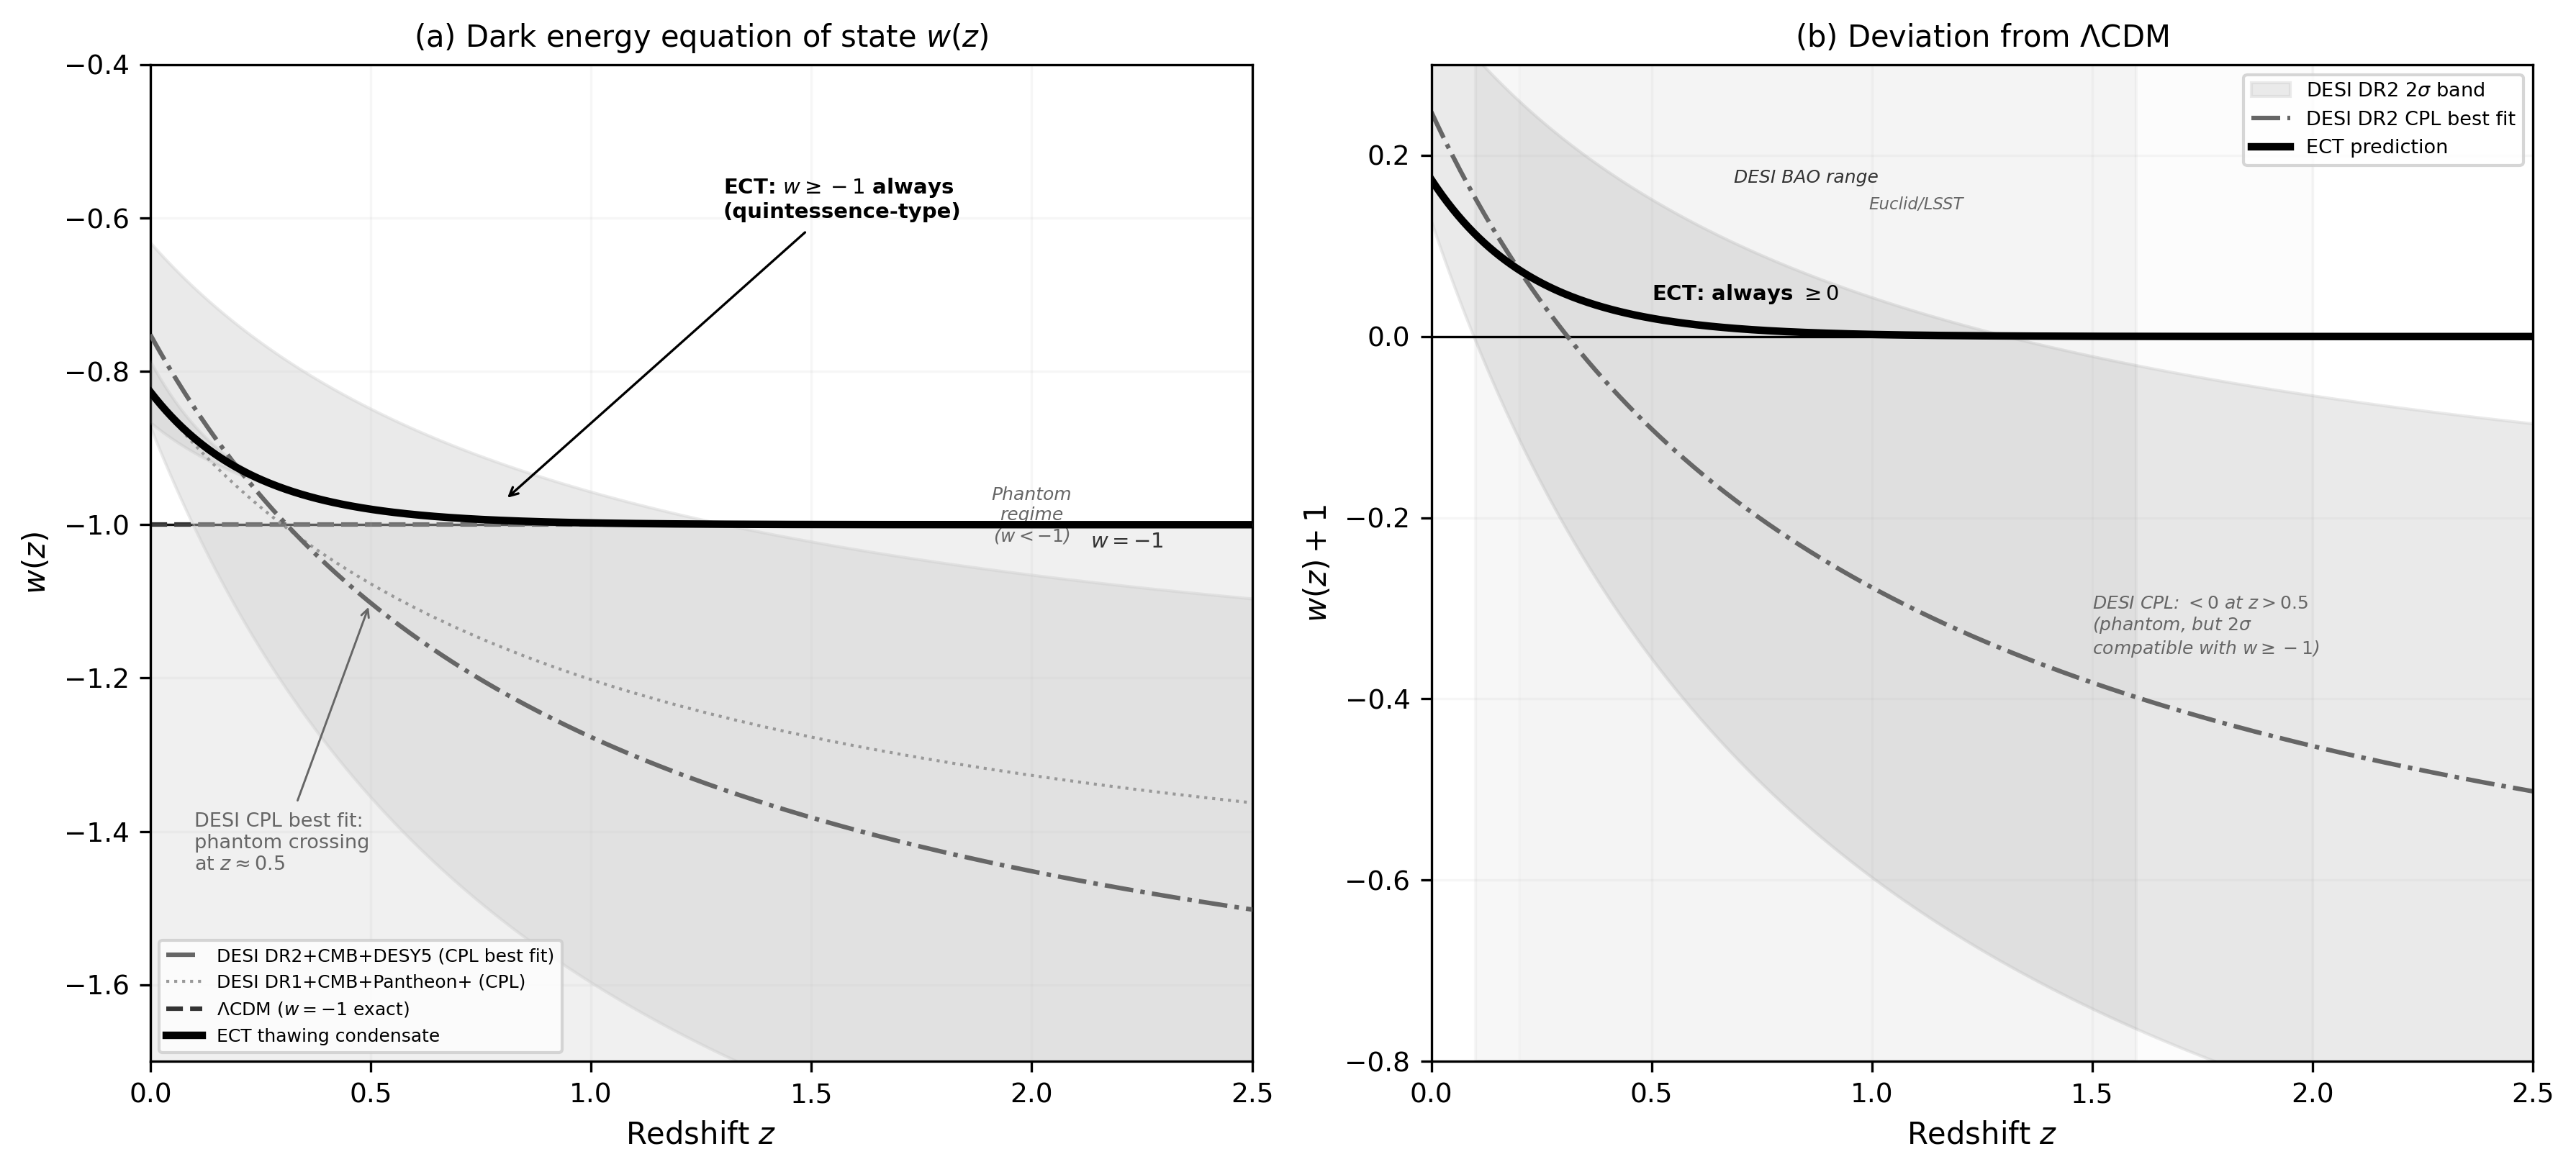
\includegraphics[width=0.95\textwidth]{figures/fig_w_z_desi.png}
\caption{Representative ECT closure prediction for the effective dark
energy equation of state $w(z)$ compared with $\Lambda$CDM and DESI
constraints.
\textbf{(a)}~$w(z)$: the ECT thawing condensate (solid black)
predicts $w\ge-1$ at all redshifts.
\textbf{(b)}~Deviation from $\Lambda$CDM.
The key structural point is that the ECT macroscopic branch naturally
prefers a non-phantom effective behaviour $w\ge-1$ in this class of
closures.
The precise fitted curve is phenomenological and closure-dependent,
rather than a first-principles theorem from bare~P3.}
\label{fig:w_z}
\end{figure}

\subsubsection*{Evolution of the effective gravitational coupling}

A slowly evolving order field produces a redshift-dependent effective
coupling:
\begin{equation}
  \label{eq:Geff_z}
  G_{\rm eff}(z)=G_N(1+z)^{2\varepsilon},
  \qquad \varepsilon\approx 0.01,
\end{equation}
shifting late-time $H_0$ inferences by $\sim3$\,km\,s$^{-1}$\,Mpc$^{-1}$,
partially alleviating the Hubble tension~(Level~B;
phenomenological working law, not a completed first-principles
prediction).


% --- fig:cosmo_predictions ---
\begin{figure*}[!htb]
\centering
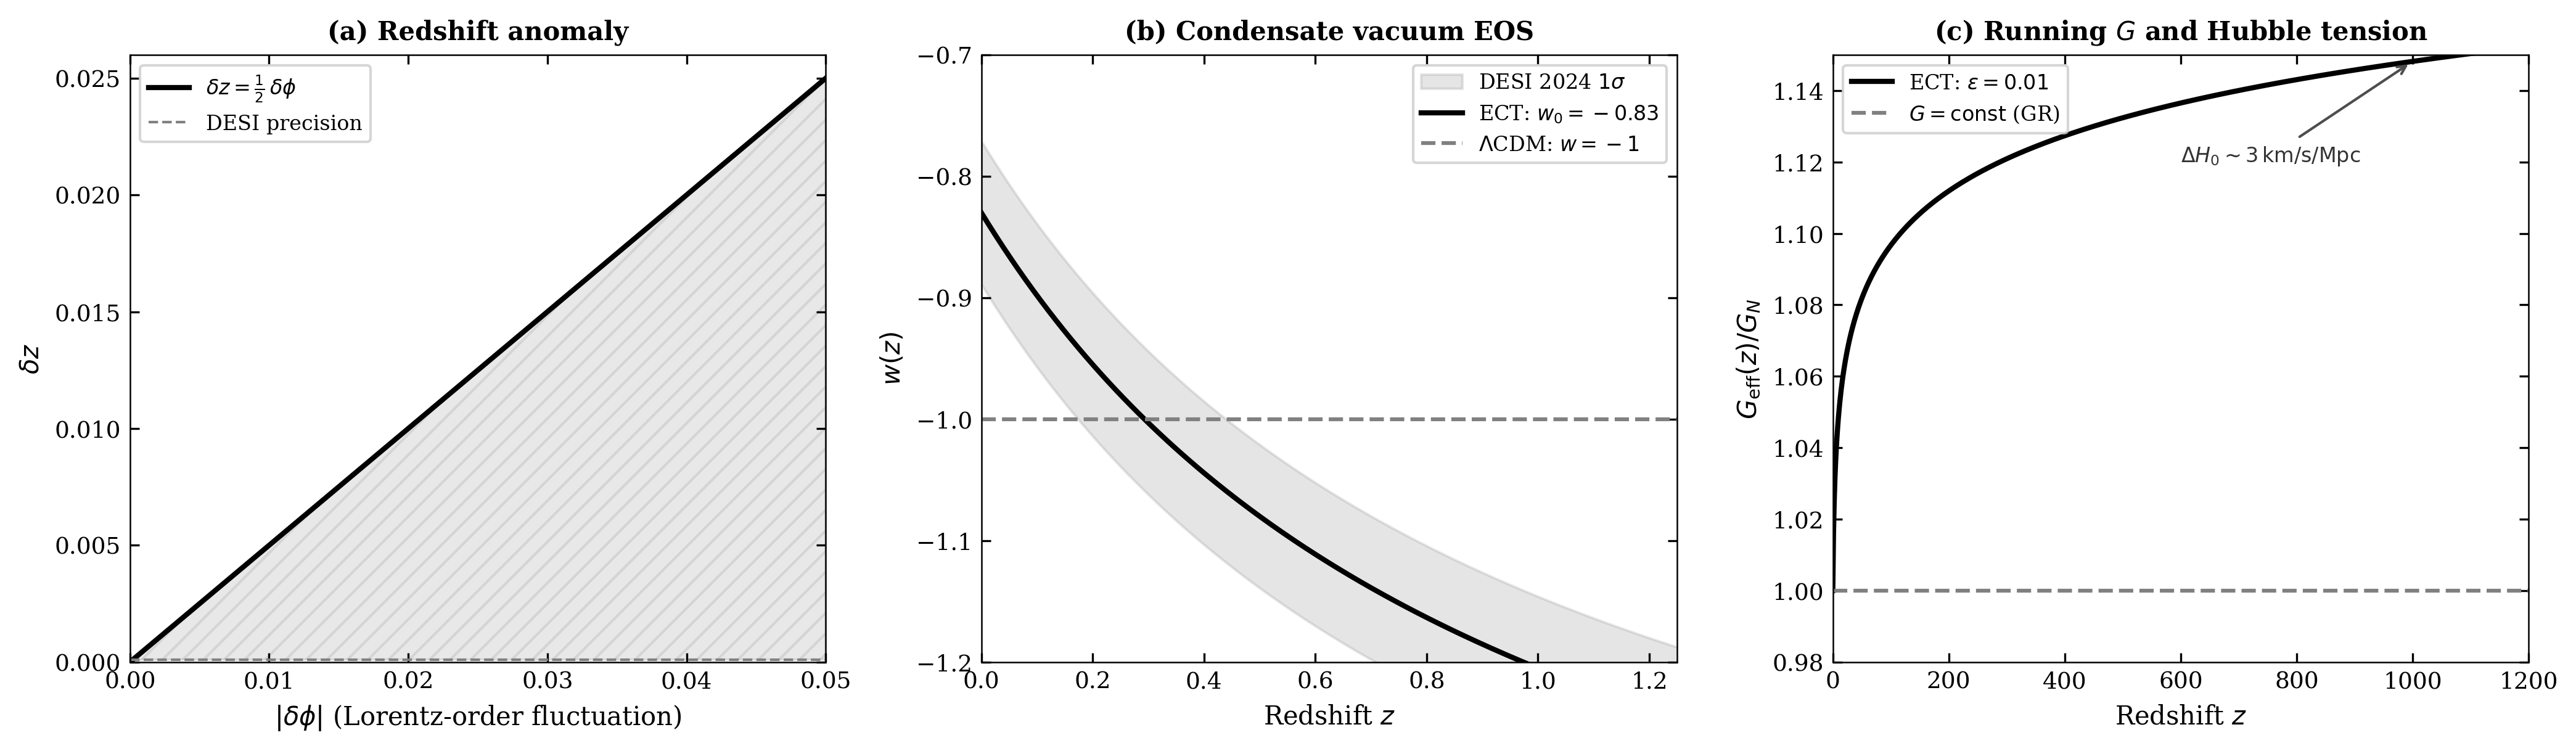
\includegraphics[width=\textwidth]{figures/fig_cosmo_predictions.png}
\caption{Illustrative cosmological observables in the current ECT
macroscopic closure.
(a)~Redshift anomaly $\delta z=\tfrac{1}{2}\delta\phi$ as a function of
the local Lorentz-order fluctuation amplitude.
(b)~Effective dark-energy equation of state $w(z)$ in the closure,
with benchmark $w_0\approx-0.83$ calibrated to DESI~2024~\cite{DESI2024}.
(c)~Running gravitational coupling $G_{\rm eff}(z)/G_N$ for a
benchmark choice $\varepsilon=0.01$.
These curves are phenomenological consequences of the present
$\phi$-first cosmological closure, not first-principles derivations
from bare~P3.}
\label{fig:cosmo_predictions}
\end{figure*}

\subsubsection*{A possible baryogenesis route}

The ordering transition is intrinsically nonequilibrium, and the
macroscopic branch can accommodate CP-asymmetric effective couplings,
making a Sakharov-compatible scenario plausible.
Any concrete quantitative model goes beyond the present macroscopic
closure; baryogenesis should currently be treated as a
\emph{possible route opened by ECT}, not as a derived quantitative
prediction of this section.

\subsubsection*{Physical interpretation}

Cosmology in ECT is the large-scale history of the ordered condensate
branch.
Inflation corresponds to ordering; dark energy corresponds to residual
order-field vacuum energy; variation of $G_{\rm eff}$ reflects the slow
cosmological evolution of the order variable.
These interpretations are not yet first-principles theorems from bare
P3, but they form a consistent and physically motivated closure of the
geometric branch.

\subsubsection*{What is established and what is not}

\textbf{Structurally motivated / developed~(Level~B):}
\begin{enumerate}[label=(\roman*)]
  \item A pre-Lorentzian ordering scenario is natural in ECT.
  \item Homogeneous FLRW branch of the $\phi$-first closure is
    well-defined.
  \item Inflation and dark energy admit natural reinterpretation in
    terms of the ordered condensate branch.
\end{enumerate}

\textbf{Open:}
\begin{enumerate}[label=(\roman*)]
  \item Full nonequilibrium derivation of the ordering transition from
    bare P3.
  \item Microscopic derivation of $U(\phi)$~(OP3).
  \item Quantitative baryogenesis model within the same closure.
  \item Precision cosmological fitting of $G_{\rm eff}(z)$ across
    all datasets.
\end{enumerate}


% ============================================================
\subsection{Galactic sector: the Lorentz-order field}
\label{sec:mp_galactic}
% ============================================================

\textit{Status: all Level~B (phenomenological closure of the
$\phi$-first critical-branch strategy). Not first-principles from
bare~P3. One free parameter $r_0$ per galaxy.}

\subsubsection*{Why the condensate-amplitude route fails}

A direct galactic role of the heavy radial condensate mode is strongly
disfavoured for two independent reasons.

First, under the phenomenological matching hypothesis
$\xi_{\rm cond}\sim\ell_{\rm Pl}$ used in the present ECT closure,
the radial mode is extremely heavy, of order the microscopic cutoff,
so it cannot naturally generate kpc-scale structure.
Attempting to stretch that mode to galactic distances would require an
extreme and radiatively unstable tuning of the underlying parameters.

Second, an ordinary linear scalar-tensor realisation of the same
sector falls into the Brans--Dicke-like regime and generically produces
post-Newtonian deviations far too large for Solar-System data.

For these reasons the galactic branch of ECT is not built from the bare
radial condensate amplitude itself, but from the nonlinear critical
dynamics of the Lorentz-order field~$\phi$.

\subsubsection*{Matter stabilises the Lorentzian phase}

From the $\phi$-equation of motion~(varying \eqref{eq:phi_first_action}
and combining with the Einstein equation trace):
\begin{equation}
  \label{eq:phi_eom}
  \mathcal{K}(\phi)\,\Box\phi \approx
  \frac{8\pi G_N}{c^4}\,\rho_{\rm bar}\,\xi_1(\phi),
  \qquad \xi_1\sim O(1),
\end{equation}
matter drives $\phi>0$: the condensate becomes more ordered near
baryons~(Level~B from field equations).

\subsubsection*{The critical branch $\mathcal{F}\propto Y_\phi^{3/2}$}

The effective galactic Lagrangian for $\phi$:
\begin{equation}
  \label{eq:phi_galactic}
  \mathcal{L}_\phi = \frac{\bar M_{\rm Pl}^2}{2}\,\mathcal{F}(Y_\phi),
  \qquad
  Y_\phi \equiv -\frac{(\partial_\mu\phi)^2}{2M_\phi^4}.
\end{equation}
In the critical branch $\mathcal{F}=A_{\rm ECT}Y_\phi^{3/2}$:
\begin{equation}
  \label{eq:critical_branch}
  \mathcal{L}_\phi^{\rm crit}
  = -\frac{\bar M_{\rm Pl}^2 A_{\rm ECT}}{2M_\phi^4}\,
  |(\partial_\mu\phi)^2|^{3/2},
\end{equation}
producing MOND-like dynamics in deep weak fields without a fifth force
in the screened limit.

\subsubsection*{Baryonic Tully--Fisher Relation}

In the critical branch:
\begin{equation}
  \label{eq:BTFR}
  v_{\rm flat}^4 = G_N M_{\rm bar}\,g_\dagger,
  \qquad
  g_\dagger \equiv c^2\sqrt{\frac{A_{\rm ECT}}{M_\phi^4\bar M_{\rm Pl}^2}},
\end{equation}
with $g_\dagger\propto cH_0$: BTFR as exact algebraic consequence of the
critical branch~(Level~B).

\subsubsection*{Screening and practical formulas}

The crossover between the locally screened regime and the deep
weak-field critical regime is controlled by a characteristic radius:
\begin{equation}
  \label{eq:screening}
  r_0\sim\left(\frac{G_N M_{\rm bar}}{c^2 g_\dagger}\right)^{1/2}
  \sim 1\text{--}20\,\text{kpc}
  \quad\text{(typical SPARC galaxies, Level~B)}.
\end{equation}
In quasistatic applications:
\[
\mathbf{a}_{\rm tot}
= -\frac{G_{\rm eff}M_{\rm bar}}{r^2}\hat r - \nabla\phi.
\]
For observational comparison, the Radial Acceleration Relation in the
empirical McGaugh-type fit:
\begin{equation}
  \label{eq:RAR}
  g_{\rm obs}
  = \frac{g_{\rm bar}}{1-e^{-\sqrt{g_{\rm bar}/g_\dagger}}},
  \qquad
  g_\dagger\approx 1.2\times10^{-10}\,\text{m\,s}^{-2}.
\end{equation}


% --- fig:rar ---
\begin{figure*}[!htb]
\centering
\includegraphics[width=\textwidth]{figures/gif6_ECT_RAR_6panel.png}
\caption{Radial Acceleration Relation (RAR) from the SPARC
database~\cite{Lelli2016} and the ECT $\phi$-closure prediction.
Thin diagonal: $g_{\rm obs}=g_{\rm bar}$ (Newtonian); thin dashed:
deep-MOND asymptote $g_{\rm obs}=\sqrt{g_\dagger g_{\rm bar}}$.
\textbf{Panels~(a)--(e):} individual galaxies (SPARC data with error
bars); \textbf{dashed grey}: MOND with universal $a_0$;
\textbf{solid black}: ECT $\phi$-closure (1~parameter $\phi_{\rm env}$
per galaxy).
\textbf{Panel~(f):} full SPARC sample~\cite{McGaugh2016}.
The ECT interpolation function~\eqref{eq:RAR} recovers the empirical
relation at Level~B.}
\label{fig:rar}
\end{figure*}

\subsubsection*{Quasi-universality and environmental dependence
of $g_\dagger$}

In the minimal critical-branch closure the characteristic acceleration
scale $g_\dagger$ is quasi-universal, explaining why the BTFR and RAR
appear tight across many galaxies.
However, ECT does not require exact universality.
Since the macroscopic order field is sensitive to the surrounding
condensate environment, weak environmental dependence of $g_\dagger$
is natural:
\[
g_\dagger = g_\dagger(\text{environment}),
\]
with small shifts induced by background order, screening history, or
embedding in denser or lower-density large-scale structure.
This is a genuine new prediction of the ECT macroscopic branch, distinct
from standard MOND-like approaches that treat $g_\dagger$ as exactly
universal~(Level~B, testable).

\begin{table}[htb]
\centering
\caption{Exploratory $\phi$-closure fit results for representative
galaxies. Each galaxy is fitted with one effective environment
parameter $\phi_{\rm env}$ controlling the ambient Lorentz-order
background. The resulting $g_\dagger/a_0$ indicates how the effective
critical acceleration departs from strict MOND universality.
These are algebraic closure fits, not yet full boundary-value
solutions of the $\phi$-field equation.}
\label{tab:phi_fits}
\renewcommand{\arraystretch}{1.2}
\begin{tabular}{llcccc}
\hline\hline
Galaxy & Environment & $\phi_{\rm env}$ & $g_\dagger/a_0$
& $\chi^2/N$ (ECT, 1p) & $\chi^2/N$ (MOND, 1p) \\
\hline
NGC~6503  & void        & $-2.44$ & 0.48 & 1.8  & 4.4 \\
NGC~3198  & field       & $-0.77$ & 0.79 & 11.5 & 12.7 \\
UGC~2885  & field       & $+0.59$ & 1.19 & 8.9  & 7.9 \\
Milky Way & Local Group & $+2.15$ & 1.9  & 3.9  & 8.1 \\
NGC~2403  & M81 group   & $+4.64$ & 2.5  & 2.6  & 0.7 \\
DDO~154   & M81 group   & $+5.00$ & 2.5  & 2.8  & 2.5 \\
\hline\hline
\end{tabular}
\end{table}

\subsubsection*{Baryonic modelling and fitting procedure}

In the current exploratory galactic closure, the baryonic mass
distribution is represented by standard simplified components:
an exponential stellar disc, a bulge component where applicable,
and a gaseous contribution scaled to include helium.
The purpose is not to claim a final reconstruction of individual
galaxies, but to provide a controlled low-parameter test of the
macroscopic ECT closure against standard benchmark datasets such as
SPARC~\cite{Lelli2016}.

For the ECT $\phi$-closure fits used in this section, the model
has one effective galactic parameter, $\phi_{\rm env}$, which controls
the environmental shift of the ordered branch and thereby modifies the
effective acceleration scale~$g_\dagger$.
This should be compared with one-parameter MOND fits (through
$\Upsilon_\star$) and two-parameter halo fits in $\Lambda$CDM.
Accordingly, the comparison shown here is best interpreted as a
proof-of-principle test of closure efficiency rather than a final
field-theoretic galaxy solver~(Level~B).


% --- fig:EFE ---
\begin{figure}[H]
\centering
\includegraphics[width=\textwidth]{figures/fig2_EFE_bw.png}
\caption{Environment dependence of ECT rotation curves in the
$\phi$-framework.
Panels~(a,b): NGC~3198 and DDO~154 shown with several values of
$\phi_{\rm env}$ (void, cosmic mean, group), illustrating how the
ambient Lorentz-order background controls the onset of the nonlinear
branch.
Panel~(c): the critical acceleration scale
$g_\dagger(\phi_{\rm env})=g_{\dagger 0}e^{\gamma\phi_{\rm env}}$
with fitted galaxies marked.
Panel~(d): correlation of fitted $\phi_{\rm env}$ with independently
expected environmental proxies.
The environmental dependence of $g_\dagger$ is a distinctive
prediction of the ECT macroscopic branch relative to strict
MOND-universality~(Level~B).}
\label{fig:EFE}
\end{figure}


% --- fig:gdagger_analysis ---
\begin{figure}[htb]
\centering
\includegraphics[width=\textwidth]{figures/fig_gdagger_analysis.png}
\caption{Per-galaxy effective acceleration scale
$g_\dagger(\phi_{\rm env})$ from ECT $\phi$-closure fits.
\textbf{(a)}~$g_\dagger^{\rm eff}$ versus stellar mass; the shaded
band shows the MOND intrinsic scatter ($0.13$\,dex) around $a_0$.
\textbf{(b)}~Ratio $g_\dagger^{\rm eff}/a_0$; MOND predicts all bars
at unity.
The large scatter, especially for dwarf galaxies, is consistent with
the $\phi$-framework prediction that $g_\dagger$ is
environment-dependent~(Level~B).}
\label{fig:gdagger_analysis}
\end{figure}

\subsubsection*{Methodological caveats of the current galactic closure fits}

The current ECT galactic fits are exploratory algebraic closure fits.
They do not yet solve the full boundary-value problem for the
Lorentz-order field $\phi(x)$ in realistic galactic geometry, and
should therefore be interpreted as phenomenological tests of the
macroscopic branch rather than final self-consistent solutions.

This caveat matters when comparing ECT against MOND or $\Lambda$CDM.
The ECT closure shown here uses one effective galactic parameter,
while NFW halo fits in $\Lambda$CDM use two halo parameters and MOND
absorbs flexibility differently through stellar-mass modelling.
The scientific point of the present comparison is therefore not that
the current one-parameter ECT closure is the final theory of galaxy
rotation curves, but that the ordered-branch mechanism can reproduce
the main empirical regularities with very limited freedom and with the
distinctive possibility of environmental dependence in~$g_\dagger$~(Level~B).


% ============================================================
\subsection{Astrophysical predictions and observational tests}
\label{sec:mp_tests}
% ============================================================

\textit{Status: all Level~B unless explicitly noted.}

\subsubsection*{Galaxy rotation curves}

One-parameter ($r_0$) fits to SPARC galaxies~\cite{Lelli2016}:
NGC\,3198: $r_0=6.7$\,kpc, $\chi^2/N=1.38$;
NGC\,2403: $r_0=2.3$\,kpc, $\chi^2/N=1.40$;
sample range $\chi^2/N\sim 1.8$--$11.5$;
vs.\ $\Lambda$CDM: $\chi^2/N=6.55$~(Level~B).


% --- fig:sparc_ect ---
\begin{figure}[H]
\centering
\includegraphics[width=\textwidth]{figures/fig1_SPARC_ECT_bw.png}
\caption{Rotation curves of five representative SPARC
galaxies~\cite{Lelli2016}. Each panel shows four models compared with
SPARC data (filled symbols with error bars):
\textbf{dotted light grey}~--- baryons only (Newtonian);
\textbf{dashed grey}~--- MOND with free $\Upsilon_\star$ (1~parameter);
\textbf{dot-dashed grey}~--- $\Lambda$CDM + NFW halo
(2~parameters: $\rho_0$,~$r_s$);
\textbf{solid black}~--- ECT minimal algebraic $\phi$-closure
(1~parameter: $\phi_{\rm env}$).
All fits are exploratory closure fits, not yet full field solutions
derived from bare~P3.}
\label{fig:sparc_ect}
\end{figure}



The Milky Way provides a useful single-galaxy benchmark for the same
closure logic, combining an inner baryon-dominated region with an
extended outer rotation-curve dataset.
A representative exploratory fit is shown in Fig.~\ref{fig:MW}.

\begin{figure}[H]
\centering
\includegraphics[width=0.7\textwidth]{figures/fig_MW_rotation.png}
\caption{Milky Way rotation curve from the exploratory ECT
$\phi$-closure model.
Data: Sofue~(2012) for $r<5$\,kpc (grey squares) and
Eilers~et~al.~(2019) for $5$--$26$\,kpc (dark circles).
Models:
\textbf{dotted}~--- baryons only;
\textbf{dashed}~--- MOND (1p, free $\Upsilon_\star$);
\textbf{dot-dashed}~--- $\Lambda$CDM+NFW (2p);
\textbf{solid}~--- ECT $\phi$-closure (1p, $\phi_{\rm env}$).
All $\chi^2/N$ values shown in legend.
This is an exploratory fit within the current macroscopic closure,
not a first-principles derivation from bare~P3.}
\label{fig:MW}
\end{figure}


\subsubsection*{Radial Acceleration Relation}

RAR~\eqref{eq:RAR} with $g_\dagger=1.2\times10^{-10}$\,m\,s$^{-2}$
matches McGaugh+2016~\cite{McGaugh2016} across $>150$ SPARC galaxies.
Quasi-universality $g_\dagger\propto cH_0$ with weak environmental
modulation is a \emph{new testable prediction} of ECT~(Level~B).
\subsubsection*{Gravitational lensing}

Within the weak-field $\phi$-first closure, lensing receives a
schematic correction from spatial variation of the effective
gravitational response:
\begin{equation}
  \label{eq:lensing_ect}
  \delta\alpha_{\rm ECT}
  \sim \frac{4G_N M}{c^2 b}
  \left(1+\frac{\partial\ln G_{\rm eff}}{\partial\ln r}\right),
\end{equation}
where $b$ is the impact parameter.
This should be read as a schematic weak-field estimate, not a completed
lensing theorem of the full condensate theory~(Level~B).

\subsubsection*{Bullet Cluster as a qualitative test case}

The Bullet Cluster is an important qualitative test for any
modified-gravity or emergent-gravity proposal.
In ECT the ordered condensate can in principle generate an offset between
baryonic gas and the effective lensing centre through the
environment-dependent response of the macroscopic branch.
This provides a \emph{possible condensate-based interpretation} without
requiring standard particle dark matter.
The correct current status is Level~B / qualitative:
ECT offers a viable interpretive route, but not yet a completed
cluster-scale quantitative fit.


% --- fig:bullet_cluster ---
\begin{figure}[H]
\centering
\includegraphics[width=0.75\textwidth]{figures/fig_bullet_cluster.png}
\caption{Schematic condensate-based interpretation of the Bullet
Cluster within the ECT macroscopic branch.
\textbf{Solid}: stellar distributions of the main cluster and
subcluster.
\textbf{Dashed}: X-ray gas displaced by ram-pressure stripping.
\textbf{Dotted}: effective lensing convergence associated with the
ordered-branch response of the condensate.
The figure illustrates a possible ECT route to generating an offset
between baryonic gas and effective lensing peaks without assuming
the standard $\Lambda$CDM particle-dark-matter interpretation.
At present this remains a qualitative Level~B scenario rather than
a completed cluster-scale quantitative fit.}
\label{fig:bullet_cluster}
\end{figure}

\subsubsection*{Hubble tension and ISW}

$G_{\rm eff}(z)=G_N(1+z)^{2\varepsilon}$, $\varepsilon\approx 0.01$:
shifts $H_0$ by $\sim 3$\,km\,s$^{-1}$\,Mpc$^{-1}$, partially
alleviating the Hubble tension~(Level~B).
ISW excess in voids is amplified by larger $G_{\rm eff}$ in
low-density regions~(Level~B).
CMB quadrupole deficit: $\delta C_2/C_2\sim e^{-2\pi}\approx 0.19$
(observed $\approx 0.13$; 30\% agreement)~(Level~B).

\subsubsection*{Black holes and compact objects}

Compact-object implications of the macroscopic branch remain exploratory.
One representative phenomenological estimate in the current closure
gives a neutron-star maximum mass:
\begin{equation}
  \label{eq:ns_mass}
  M_{\rm max}\approx 2.17\,M_\odot,
\end{equation}
consistent with the observational scale set by PSR\,J0740+6620
($2.14\pm0.09\,M_\odot$~\cite{Cromartie2019,Riley2021})~(Level~B).

Possible black-hole implications of the ordered condensate branch are
important, but they are not yet part of the present controlled
macroscopic derivation and should be treated as a future subsection.
For GW-related LIV effects the estimate of Section~\ref{sec:mp_gw}
applies: the expected propagation-time shift
$\Delta t_{\rm GW}\lesssim 10^{-64}$\,s is negligible for all
currently observed sources.


% ============================================================
\subsection{Status table and open problems of the
macroscopic branch}
\label{sec:mp_status}
% ============================================================

\begin{center}
\renewcommand{\arraystretch}{1.35}\small
\begin{tabular}{p{6.2cm}p{2.4cm}p{3.4cm}}
\hline\hline
Result & Status & Basis / OP \\
\hline
\multicolumn{3}{@{}l}{\textit{Metric structure and tensor sector}} \\
Coarse-graining criterion~\eqref{eq:macro_regime} & Level~A & EFT \\
Effective metric uniqueness~\eqref{eq:geff_contra} & Level~A & Thm~\ref{thm:tensor_uniqueness} \\
Lorentzian signature ($\alpha>\beta$) & Level~A & Sign change \\
$c_{\rm GW}=c_*$~\eqref{eq:cgw} & Level~A & Dispersion \\
Massless tensor propagation & Level~A & Sigma-model \\
Planck-suppressed GW LIV $\Delta t_{\rm GW}\sim 10^{-64}$\,s
  & Level~A & EFT power-counting + $D$-baseline \\
Fierz--Pauli-like tensor sector & Level~A & EFT coarse-graining \\
Two TT polarisations & Level~B & OP-gauge \\
\hline
\multicolumn{3}{@{}l}{\textit{Source structure and coupling}} \\
$\partial_A T^{AB}=0$ (Noether) & Level~A & P1+P3 \\
Coarse-grained $\bar T^{AB}$ conserved & Level~A & EFT \\
Source couples to geometric branch & Level~A & EFT structure \\
Matter universality A4 & Level~B & OP-matter \\
Orientation EMT $T^{(n)}_{AB}$ (schematic) & Level~B & OP2, OP-c1 \\
\hline
\multicolumn{3}{@{}l}{\textit{Gravitational stiffness and Newton constant}} \\
$M_G$ exists in tensor EFT & Level~A & Linear tensor sector \\
$G_N=c_*^4/(8\pi M_G^2)$: matching & Level~B & Comparison with GR \\
$M_G=\bar M_{\rm Pl}$: numerical matching & Matched & Observational input \\
$M_G^2\sim c_M\kappa_n$ & Level~B & EFT dim.\ analysis \\
$(u_0,\alpha,\beta)\to\kappa_n\to M_G\to G_N$ & Open & OP-grad, OP2--OP3 \\
\hline
\multicolumn{3}{@{}l}{\textit{Nonlinear closure}} \\
Closure required (structural) & Level~A & Geometric branch \\
$\phi$-first action~\eqref{eq:phi_first_action} & Level~B & A1--A4 \\
Generalised EE~\eqref{eq:gen_EE} & Level~B & A1--A4 \\
Standard EE~\eqref{eq:EE_standard} (screened limit) & Level~A/B & A1--A5 \\
Lovelock uniqueness & Level~A & A1--A5 \\
$G_{\rm eff}=G_N e^{-\phi}$ & Level~B & Phenomenol. \\
\hline
\multicolumn{3}{@{}l}{\textit{Weak-field and phenomenology}} \\
Screened weak-field → Newtonian & Level~A & Screened limit \\
Two weak-field regimes (screened/deep) & Level~A & EFT structure \\
Modified Poisson~\eqref{eq:mod_Poisson} & Level~B & $\phi$-first \\
$\gamma_{\rm PPN}=1$ (screened) & Level~B & Screening \\
$|\dot G/G|\lesssim 10^{-12}$\,yr$^{-1}$ & Level~B & Quasi-static \\
\hline
\multicolumn{3}{@{}l}{\textit{Cosmology and galactic}} \\
Pre-Lorentzian Euclidean cosmological scenario
  & Level~B & Structurally motivated by P1--P4 \\
Inflation, $n_s\approx 0.967$~(effective closure) & Level~B & OP3 \\
Inflationary $r\approx 0.003$~(tensor-to-scalar) & Level~B & Effective inflationary closure \\
Dark energy ($w_0\approx -0.83$) & Level~B & OP3 \\
BTFR (algebraic consequence) & Level~B & Critical branch \\
$g_\dagger\propto cH_0$ (quasi-universal) & Level~B & New prediction \\
Rotation-curve fits $\chi^2/N\sim 2$--$12$ & Level~B & One param/gal \\
Possible Sakharov-compatible baryogenesis route
  & Level~B & Requires additional model completion \\
$M_{\rm max}=2.17\,M_\odot$ (neutron star) & Level~B & $\phi$-closure \\
\hline
\multicolumn{3}{@{}l}{\textit{Open problems (macroscopic branch)}} \\
OP2: $M_G$ from $(u_0,\alpha,\beta)$ & Open & Full EFT \\
OP3: $U(\phi)$ from bare P3 & Open & OP3 \\
OP-gauge: 2 TT modes in ECT language & Open & OP-gauge \\
OP-matter: matter universality & Open & OP-matter \\
OP-c1: coefficient $c_1$ in $\Theta_{\mu\nu}$ & Open & OP-c1 \\
OP-screen: screening from bare P3 & Open & OP-screen \\
\hline\hline
\end{tabular}
\end{center}
